\documentclass[12pt,letterpaper]{article}

\usepackage[margin=1in]{geometry}
\usepackage{amsmath,amssymb}
\usepackage{graphicx}
\usepackage{booktabs}
\usepackage{array}
\usepackage{hyperref}
\usepackage[numbers,sort&compress]{natbib}
\usepackage{setspace}
\usepackage{xcolor}
\usepackage{microtype}
\usepackage{float}
\usepackage{caption}

\hypersetup{
    colorlinks=true,
    linkcolor=blue!70!black,
    citecolor=blue!70!black,
    urlcolor=blue!70!black,
    pdftitle={The Measurement Problem Dissolved},
    pdfauthor={Heath W. Mahaffey}
}

\newcommand{\IAM}{\textsc{iam}}
\newcommand{\kB}{k_{\mathrm{B}}}
\newcommand{\QL}{Q_{\mathrm{L}}}
\newcommand{\EG}{E_{\mathrm{G}}}
\newcommand{\tauIAM}{\tau_{\mathrm{IAM}}}
\newcommand{\tauPD}{\tau_{\mathrm{PD}}}
\newcommand{\LCDM}{$\Lambda$CDM}

\begin{document}
\doublespacing

\begin{titlepage}
\centering
\vspace*{2cm}

{\LARGE\bfseries The Measurement Problem Dissolved:\\[0.5em]
Quantum Decoherence as Irreversible Sector Crossing\\
in the Informational Actualization Model\par}

\vspace{2cm}

{\large Heath W.\ Mahaffey\par}
\vspace{0.5cm}
{\normalsize Independent Researcher\\
Entiat, Washington 98822, USA\\
\href{mailto:hmahaffeyges@gmail.com}{hmahaffeyges@gmail.com}\par}

\vspace{1.5cm}
{\normalsize February 2026\par}

\vspace{2cm}

\begin{abstract}
\noindent
The measurement problem --- what constitutes a measurement, why does
measurement cause collapse, and what role does the observer play --- has
been debated for a century. We show that the dual-sector framework of the
Informational Actualization Model (\IAM), validated at cosmological scales
through 17 converged Planck~2018 MCMC chains ($\Delta\chi^2 = +0.54$
best-fit, $\sigma_8 = 0.800$, R-1 $< 0.01$ for all chains), dissolves
the measurement problem entirely. A measurement is any irreversible
thermodynamic interaction between a quantum system and matter that
dissipates energy $Q \geq \kB T \ln 2$ (the Landauer threshold). The
photon sector ($\Sigma = 1$) is immune to gravitational decoherence; the
matter sector ($\mu < 1$) decoheres on timescales determined by the
gravitational self-energy. No observer is required. No consciousness is
involved. We apply this criterion to the double slit experiment,
Wheeler's delayed choice, the quantum eraser, Schr\"{o}dinger's cat,
entanglement and Bell tests, Wigner's friend, and the quantum Zeno
effect. Each paradox is resolved by the same mechanism: sector crossing
through irreversible information production. We derive quantitative
predictions for each case and identify three experiments that discriminate
between \IAM{} and standard quantum mechanics using existing laboratory
infrastructure.
\end{abstract}

\vspace{1cm}
{\small\noindent\textbf{Keywords:} measurement problem, quantum
decoherence, Landauer principle, sector crossing, quantum eraser,
Wigner's friend, Bell tests, quantum Zeno effect,
Schr\"{o}dinger's cat\par}

\end{titlepage}

\section{Introduction}

Quantum mechanics is the most precisely tested theory in the history of
physics. Its predictions have been confirmed to extraordinary accuracy
across every experimental domain. Yet after a century of effort, the
theory contains a conceptual gap that has never been closed: the
measurement problem.

The standard formulation posits two distinct dynamical processes. Between
measurements, quantum states evolve unitarily according to the
Schr\"{o}dinger equation. At measurements, states undergo non-unitary
collapse to an eigenstate of the measured observable. What constitutes a
``measurement'' is not defined within the theory. Whether the observer
plays a special role remains contentious. The apparent randomness of
measurement outcomes is treated as fundamental.

We propose that this gap is closed by the Informational Actualization
Model (\IAM), a cosmological framework independently validated against
Planck~2018 and large-scale structure data~\citep{Mahaffey2026a,
Mahaffey2026repo}. \IAM's dual-sector structure --- in which photons
travel on null geodesics in a decoherence-free sector ($\Sigma = 1$)
while matter participates in irreversible gravitational processes
($\mu < 1$) --- provides a precise, quantitative criterion for when
decoherence occurs. The criterion is thermodynamic: decoherence (sector
crossing) occurs when an interaction dissipates energy $Q \geq \kB T \ln
2$, the Landauer bound for irreversible information
erasure~\citep{Landauer1961}.

This criterion resolves every foundational paradox in quantum mechanics
through the same physical mechanism. It requires no observer, no
consciousness, no special role for macroscopic apparatus, and no
modification of the quantum mechanical formalism. It simply identifies
the physical process that standard quantum mechanics leaves unnamed.

\section{The Dual-Sector Framework}

\subsection{Cosmological Origin}

At cosmological scales, \IAM{} demonstrates that matter and photons
experience different effective gravitational coupling. The modification
is governed by the activation function $E(a) = \exp(1 - 1/a)$, derived
from horizon thermodynamics, where $a$ is the cosmological scale factor.
The matter-sector coupling constant $\beta_m = \Omega_m/2$ follows from
the virial theorem. The resulting perturbation-level signature is $\mu <
1$ (suppressed gravitational growth of matter perturbations) with
$\Sigma = 1$ (photon lensing unaffected). This has been validated through
17 converged Planck~2018 MCMC chains producing $\Delta\chi^2 = +0.54$
(best-fit vs.\ \LCDM), $\sigma_8 = 0.800$, and $H_0^{\rm (matter)} =
72.26$ km\,s$^{-1}$\,Mpc$^{-1}$~\citep{Mahaffey2026a}.

\subsection{The Sector Crossing Criterion}

We define the sector crossing criterion formally. Let $S$ be a quantum
system and $D$ be a material detector (any system following a timelike
worldline). Let $Q(S,D)$ be the energy irreversibly dissipated in their
interaction, and $\QL = \kB T_D \ln 2$ be the Landauer threshold at
detector temperature $T_D$.

If $Q(S,D) < \QL$: no sector crossing occurs. $S$ remains in the
$\Sigma = 1$ sector (coherent). The interaction is thermodynamically
reversible. Quantum erasure is possible.

If $Q(S,D) \geq \QL$: sector crossing occurs. $S$ transitions to the
$\mu < 1$ sector (decohered). The interaction is thermodynamically
irreversible. Landauer entropy has been produced. Quantum erasure is
impossible.

\begin{figure}[H]
\centering
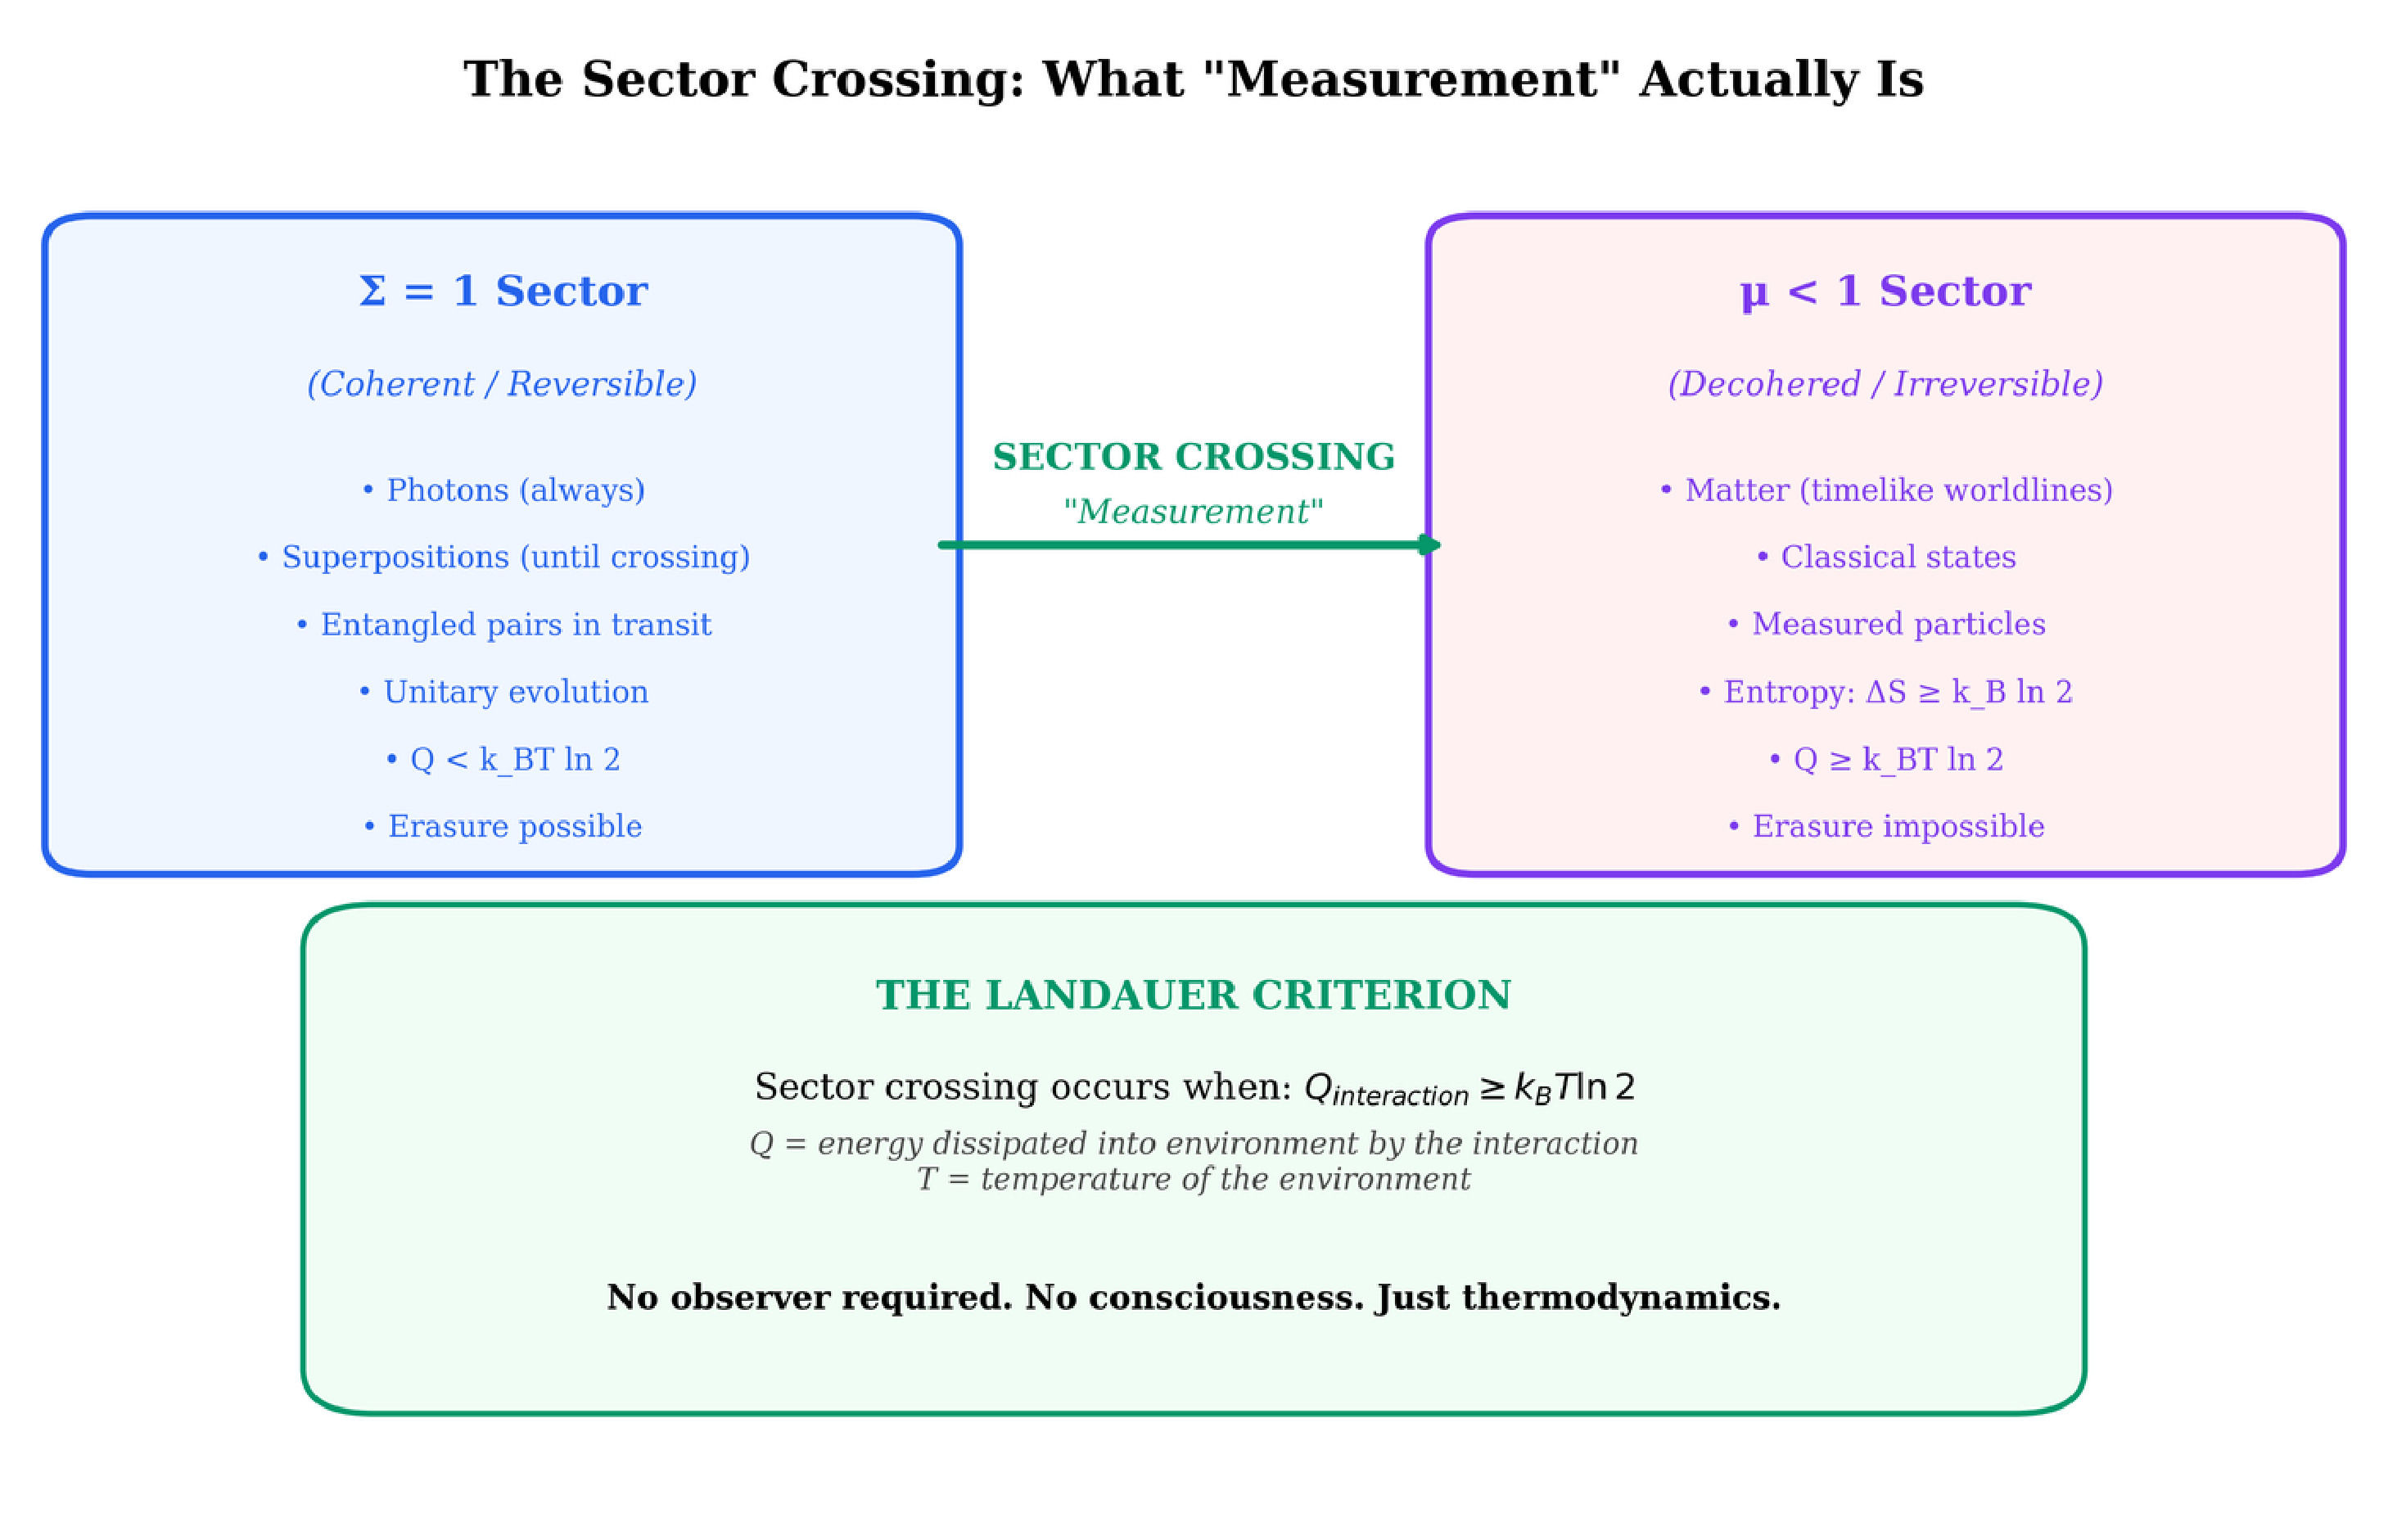
\includegraphics[width=0.88\textwidth]{fig_b1_sector_crossing.pdf}
\caption{The sector crossing criterion. The $\Sigma = 1$ sector (left,
coherent/reversible) contains photons, superpositions, and entangled
pairs in transit. The $\mu < 1$ sector (right, decohered/irreversible)
contains matter, classical states, and measured particles. Sector
crossing --- ``measurement'' --- occurs when $Q_{\rm interaction} \geq
\kB T \ln 2$. No observer required. No consciousness. Just
thermodynamics.}
\label{fig:sector}
\end{figure}

\subsection{Decoherence Timescale}

For a massive system in spatial superposition, the gravitational
self-energy $\EG = Gm^2/R$ determines the decoherence timescale.
Following the same thermodynamic derivation that produces $E(a)$ at
cosmological scales~\citep{Mahaffey2026decoherence}, the quantum-scale
decoherence timescale is:
\begin{equation}
    \tauIAM = \frac{\hbar \kB^2 T^2 \ln 2}{\EG^3}.
    \label{eq:tau}
\end{equation}
This is fully determined by mass, size, and temperature with no free
parameters. For photons, $\EG = 0$ and $\tauIAM = \infty$
(decoherence-free). For macroscopic objects, $\tauIAM$ is far below
the Planck time.

\section{Resolved Paradoxes}

\subsection{The Double Slit Experiment}

In the standard double slit experiment, a photon passes through two
slits and produces an interference pattern on a detection screen. When a
which-path detector is placed at the slits, the interference pattern
disappears. The standard interpretation attributes this to observation
collapsing the wave function.

In \IAM, the photon travels from source to slits in the $\Sigma = 1$
sector. It has $\EG = 0$ and $\tauIAM = \infty$. It is fully coherent
throughout its flight. The sector crossing occurs at the detection
screen. The screen is matter ($\mu < 1$ sector). The photon is absorbed,
an electron is excited, and irreversible information is produced
($Q \approx 2~\text{eV} \gg \QL \approx 0.018~\text{eV}$ at room
temperature). This is the collapse. Not observation. Sector crossing
through irreversible matter interaction.

When a which-path detector is placed at the slits, matter is introduced
before the screen. If the detector's interaction is irreversible
($Q > \QL$), sector crossing occurs at the slit. Coherence is lost
before the screen. No interference. If the interaction is reversible
($Q < \QL$) --- for example, a polarization rotation --- no sector
crossing occurs and interference is preserved. The human retina
($Q \approx 2.5~\text{eV}$, $Q/\QL \approx 140$) produces exactly the
same sector crossing as a CCD pixel ($Q \approx 3~\text{eV}$,
$Q/\QL \approx 170$). Consciousness plays no role.

\subsection{Wheeler's Delayed Choice Experiment}

In Wheeler's delayed choice experiment, the decision to measure wave or
particle behavior is made after the photon has passed through the slits.
The photon appears to retroactively decide whether it was a wave or
particle. This seems to require retrocausality.

\IAM{} resolves this without retrocausality. The photon is in the
$\Sigma = 1$ sector during its entire flight ($\EG = 0$,
$\tauIAM = \infty$). The flight time through a typical laboratory
apparatus (5~m) is approximately 17~ns. The decoherence accumulated
during this flight is exactly zero. The experimenter's choice of detector
configuration determines \emph{where} the sector crossing occurs, not
\emph{whether} the photon was coherent during transit. No retrocausality
is required.

\begin{figure}[H]
\centering
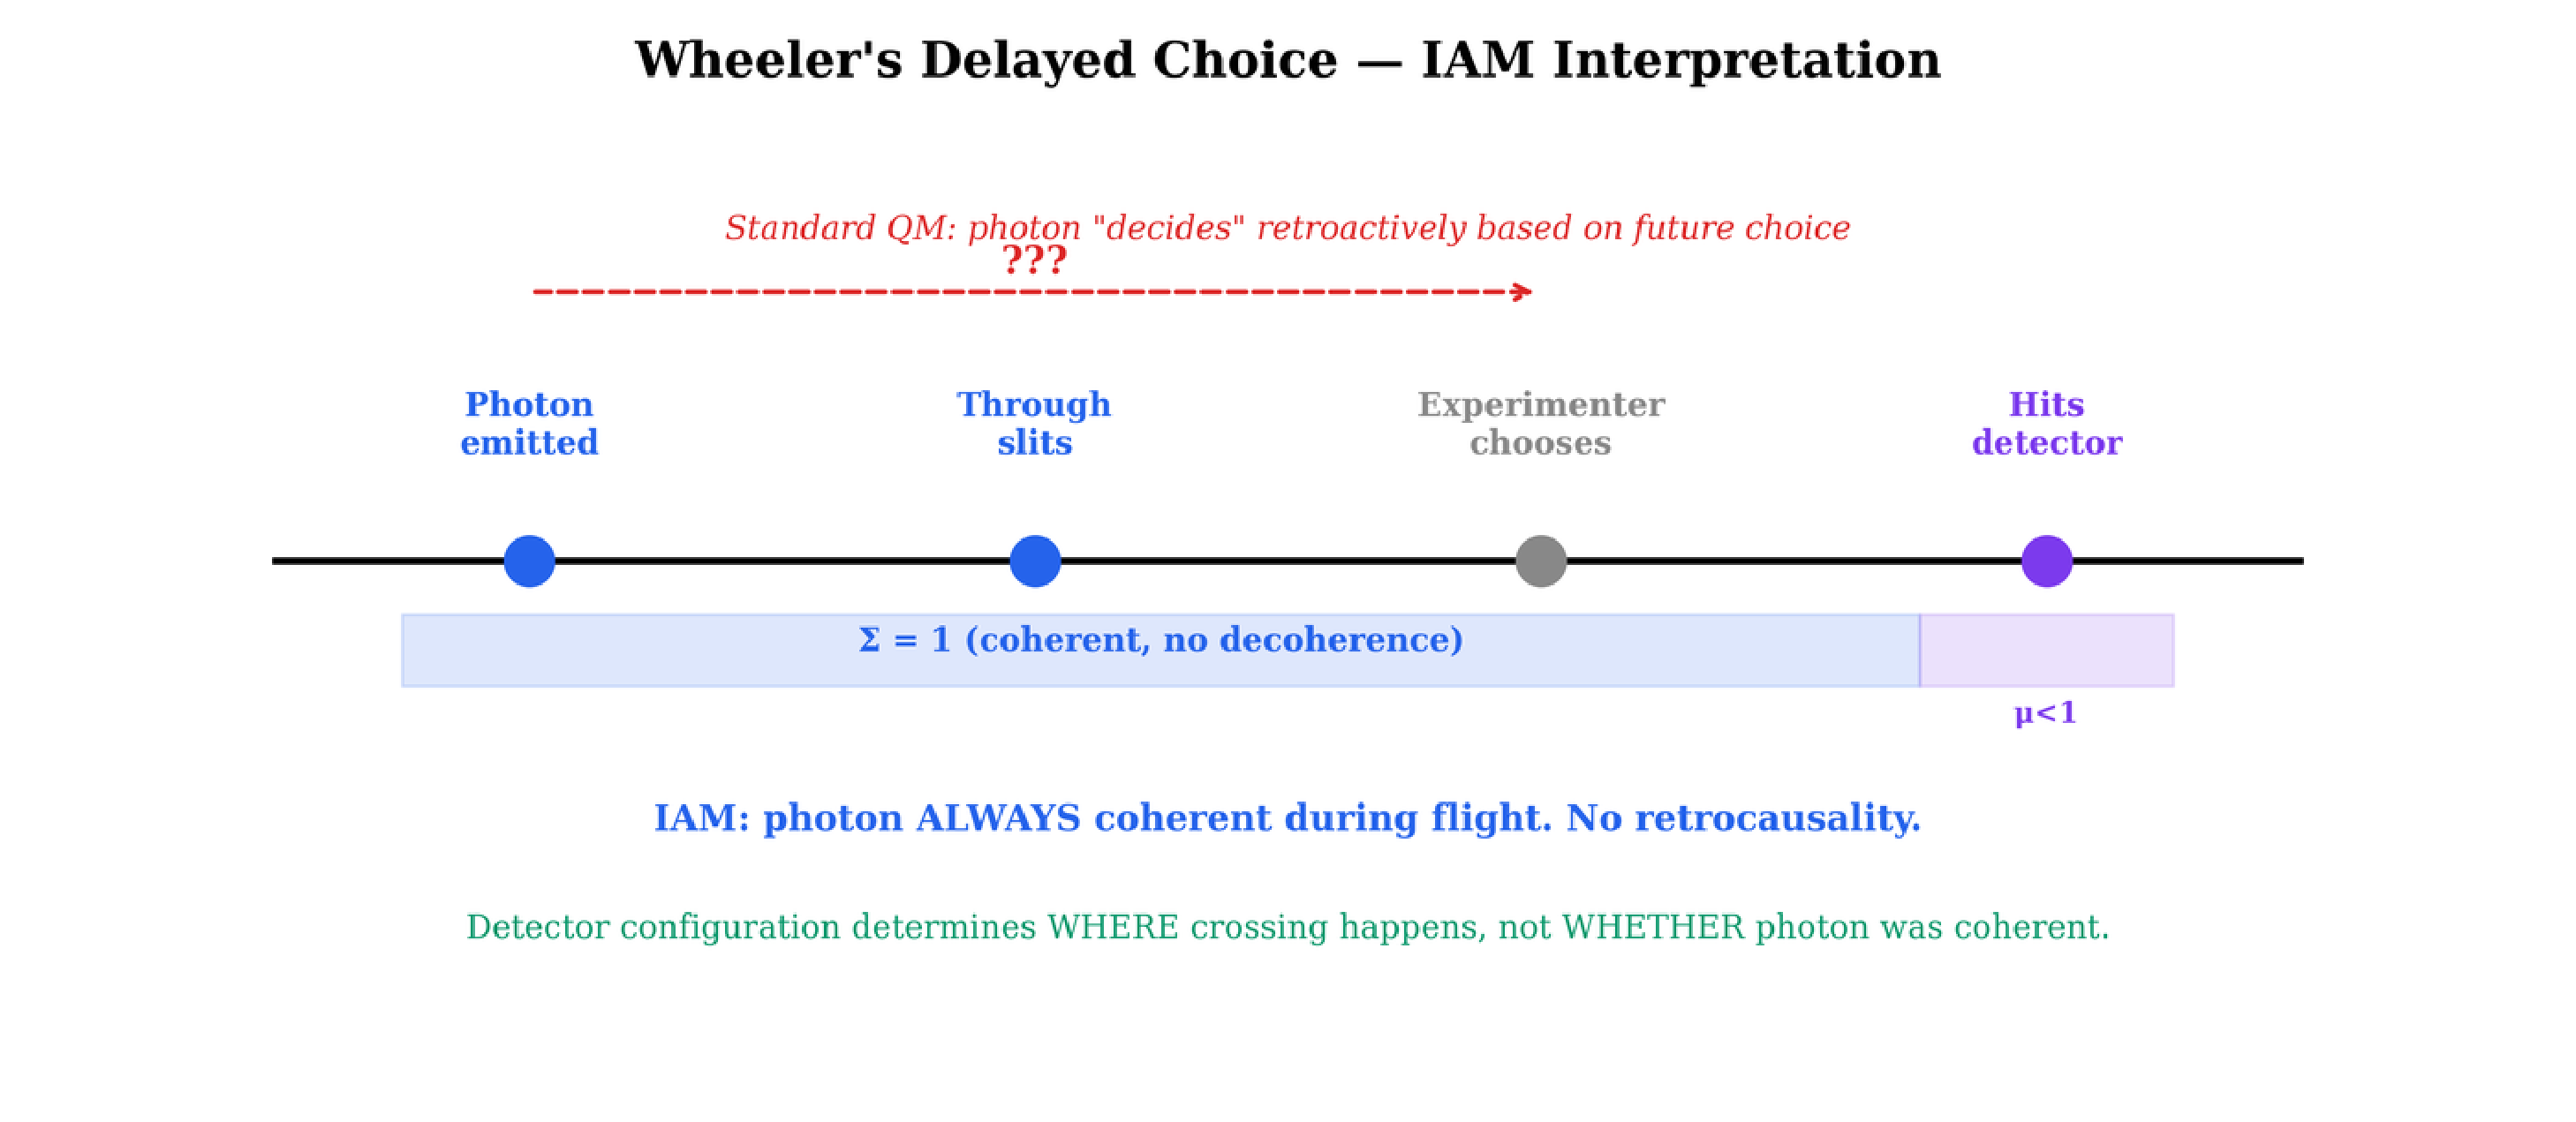
\includegraphics[width=0.88\textwidth]{fig_b3_delayed_choice.pdf}
\caption{Wheeler's delayed choice. The photon remains in the
$\Sigma = 1$ sector (coherent) throughout its entire flight. The
$\mu < 1$ crossing occurs only at the detector. The experimenter's
choice determines where the sector crossing occurs, not whether the
photon was coherent. No retrocausality is required.}
\label{fig:delayed}
\end{figure}

\subsection{The Quantum Eraser}

In quantum eraser experiments, which-path information is obtained and
then ``erased,'' and the interference pattern appears to be restored.
Standard quantum mechanics attributes this to the reversibility of
entanglement.

\IAM{} draws a critical distinction. If the which-path interaction was
thermodynamically reversible ($Q < \QL$), no sector crossing occurred.
The photon remained in the $\Sigma = 1$ sector throughout. Coherence
was never lost. The eraser reveals coherence that was always present.

If the which-path interaction was thermodynamically irreversible
($Q \geq \QL$), sector crossing occurred. Landauer entropy was produced.
The decoherence cannot be undone regardless of what operations are
performed on the ancilla. Erasure fails. We derive the erasure fidelity:
\begin{equation}
    F_{\rm IAM}(Q,T) = 1 - \frac{\exp(1 - \kB T \ln 2 / Q)}{e}.
    \label{eq:fidelity}
\end{equation}
Standard quantum mechanics predicts $F = 1$ always. \IAM{} predicts $F$
depends on $Q/\QL$. At room temperature $\QL = 0.018~\text{eV}$.
Reversible detectors (polarization rotation, beam splitters, BBO
crystals) produce $Q/\QL < 0.04$ and $F \approx 1$. Irreversible
detectors (fluorescence, photodiode, spontaneous emission) produce
$Q/\QL > 100$ and $F < 0.02$.

\begin{figure}[H]
\centering
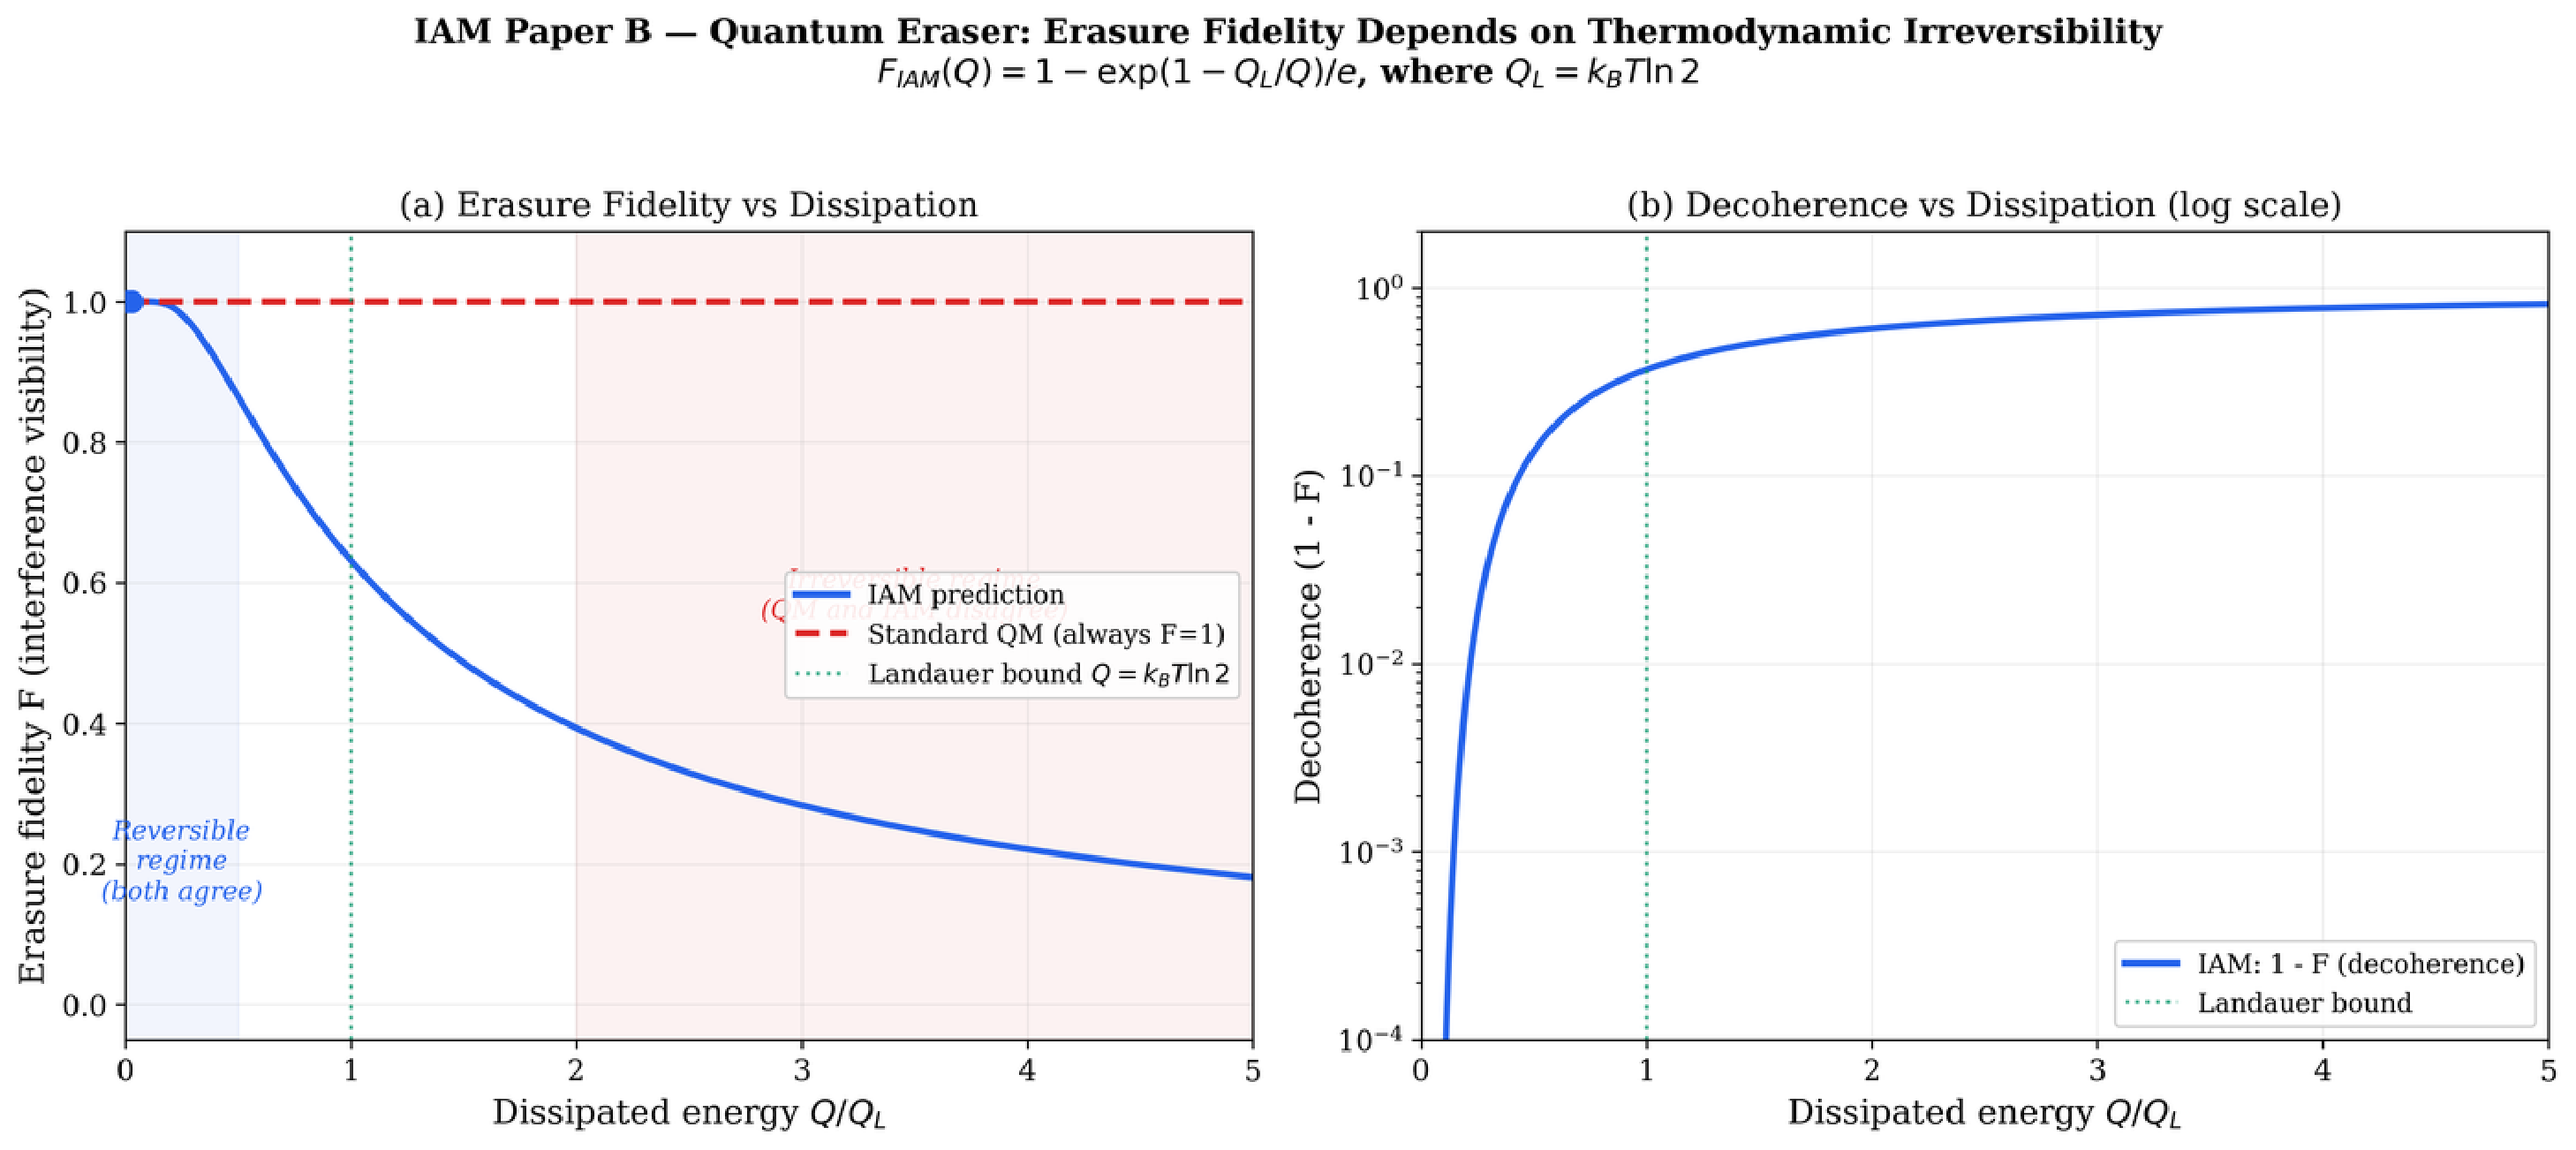
\includegraphics[width=0.88\textwidth]{fig_eraser_fidelity.pdf}
\caption{Erasure fidelity vs.\ dissipated energy $Q/\QL$.
\textbf{Left:} \IAM{} (blue) predicts fidelity falls rapidly above
the Landauer bound (green dotted). Standard QM (red dashed) predicts
$F = 1$ always. \textbf{Right:} Log-scale decoherence $1-F$. The
reversible regime ($Q < \QL$) is where both models agree; the
irreversible regime ($Q > \QL$) is where they diverge.}
\label{fig:eraser_fidelity}
\end{figure}

The most elegant experimental test uses an atomic which-path detector
with controllable spontaneous emission. Before emission ($t <
\tau_{\rm emission} \approx 10~\text{ns}$), the atomic excitation is
reversible and both models predict successful erasure. After emission
($t > \tau_{\rm emission}$), the photon has been radiated into the
environment ($Q = 2~\text{eV} \gg \QL$). \IAM{} predicts erasure
fails; standard QM predicts erasure still works if the emitted photon
is captured in a conjugate basis.

\begin{figure}[H]
\centering
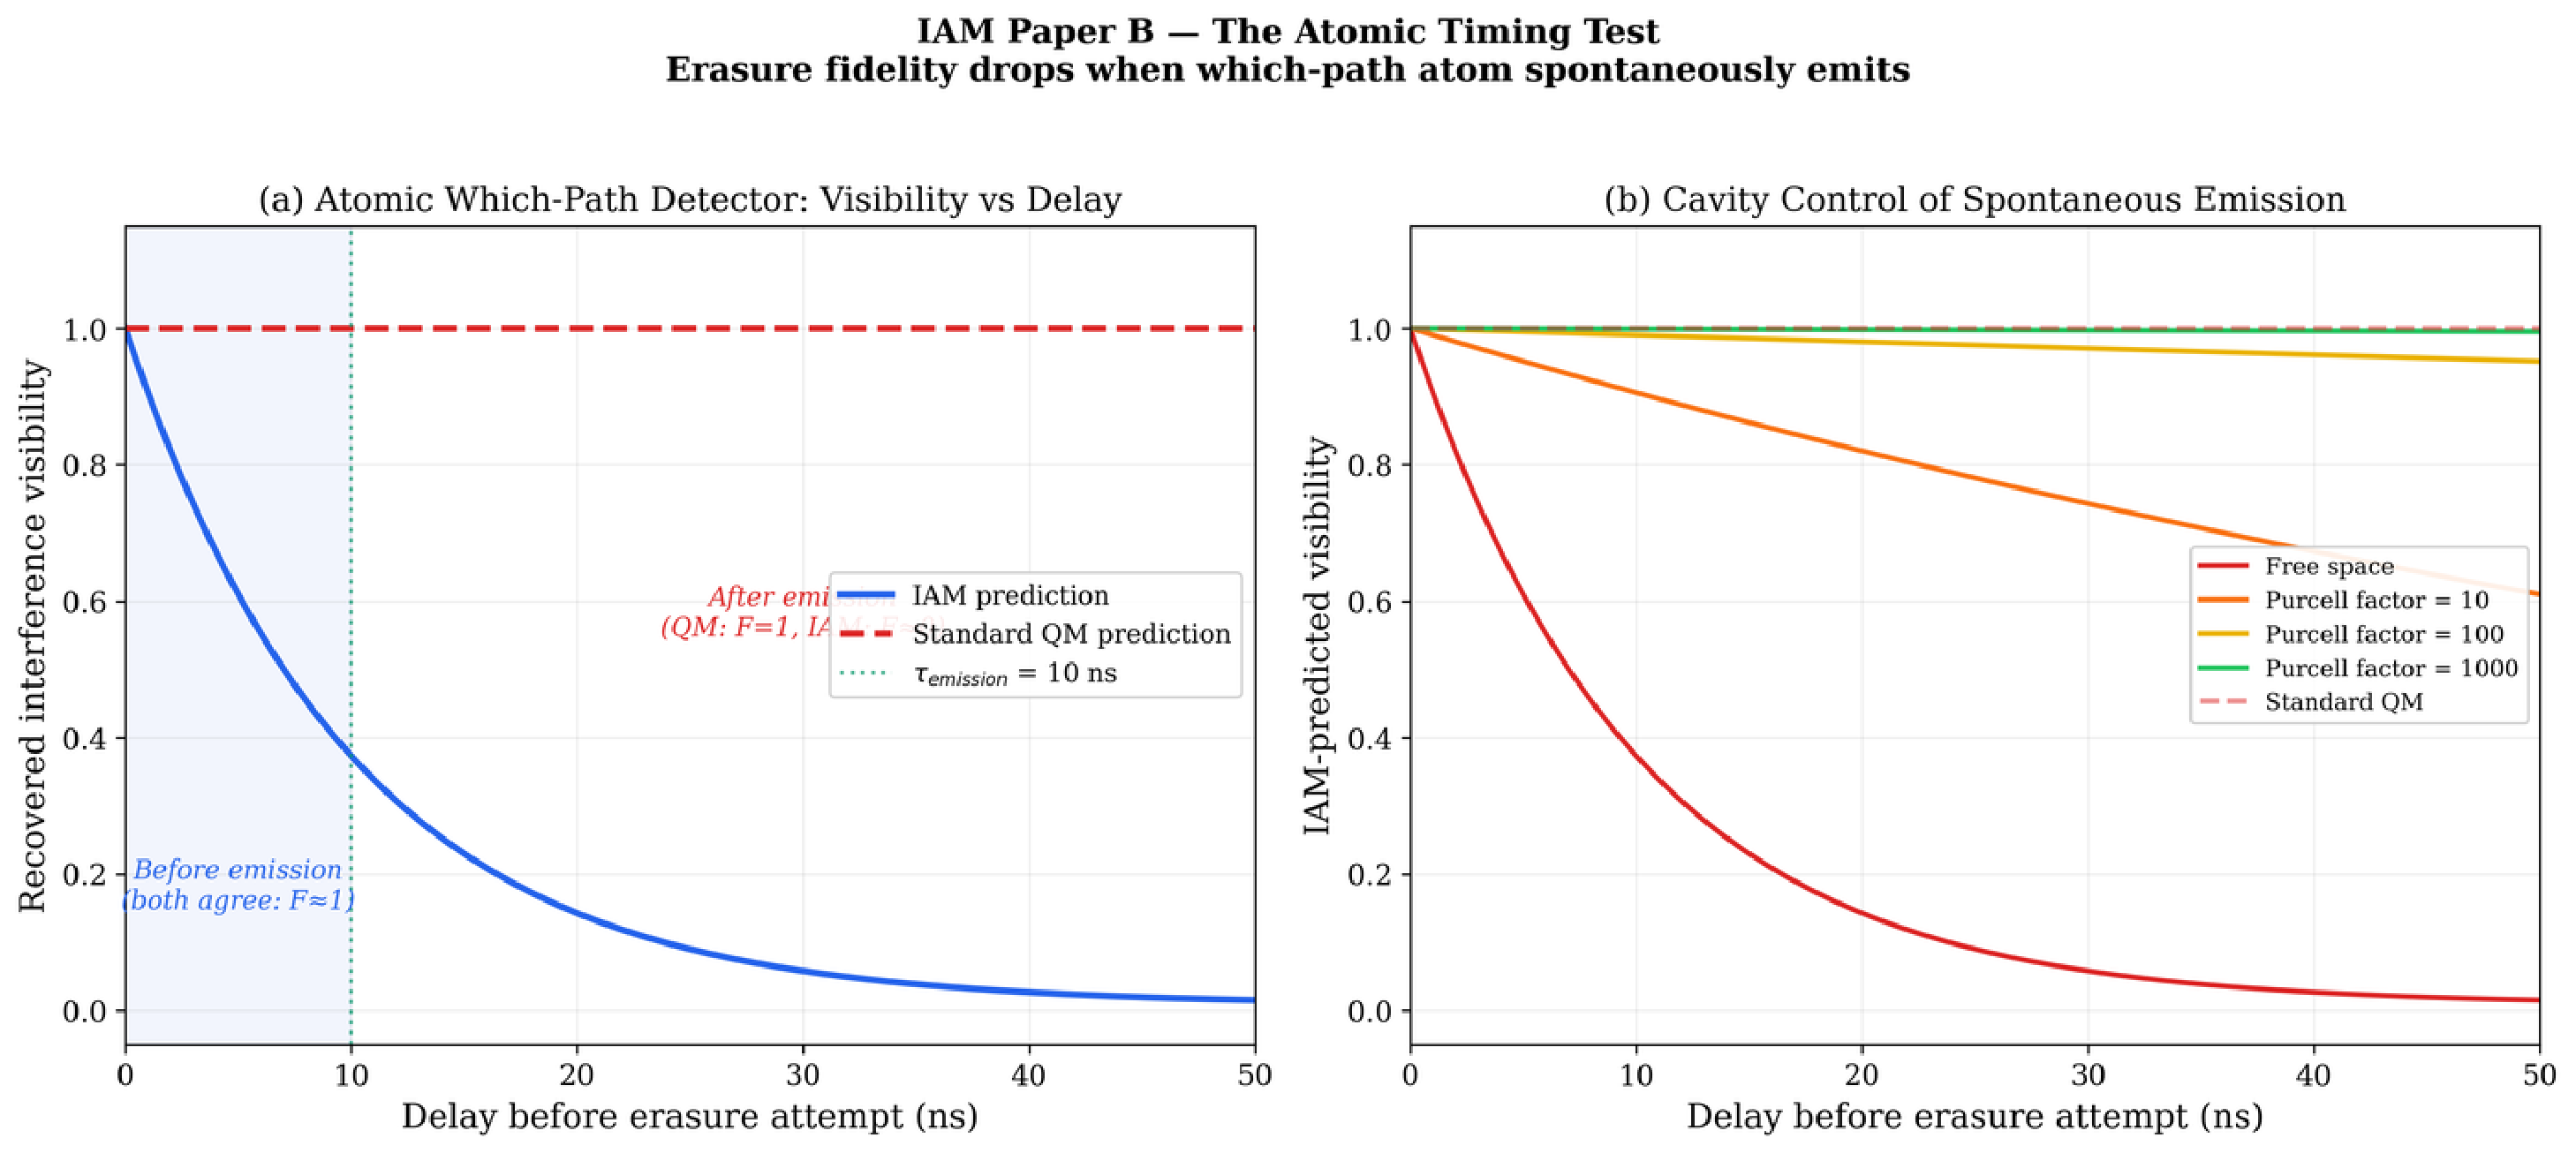
\includegraphics[width=0.88\textwidth]{fig_eraser_timing.pdf}
\caption{The atomic timing test. \textbf{Left:} Recovered interference
visibility vs.\ delay before erasure attempt. \IAM{} (blue): visibility
drops as the atom spontaneously emits at $\tau_{\rm emission} = 10$~ns.
Standard QM (red dashed): constant visibility.
\textbf{Right:} Cavity-suppressed emission (Purcell factors 1--1000)
delays the IAM-predicted drop.}
\label{fig:eraser_timing}
\end{figure}

\subsection{Schr\"{o}dinger's Cat}

Schr\"{o}dinger's thought experiment posits a cat simultaneously alive
and dead until observed. \IAM{} shows this situation is physically
impossible.

A 4~kg cat has gravitational self-energy $\EG = Gm^2/R \approx 7.1
\times 10^{-9}~\text{J}$. The \IAM{} decoherence timescale is
$\tauIAM \approx 3.7 \times 10^{-51}~\text{s}$. For reference, the
Planck time is $5.4 \times 10^{-44}~\text{s}$. The cat decoheres
approximately $10^7$~times faster than the Planck time. No physical
process could create or maintain a macroscopic superposition at this
timescale. The decoherence is not caused by observation --- it is caused
by the cat's own gravitational self-interaction.

\begin{table}[H]
\centering
\caption{Gravitational decoherence timescales from electron to human.
The mesoscopic frontier ($10^{-15}$ to $10^{-10}$~kg) is where \IAM{}
predictions become experimentally testable.}
\label{tab:timescales}
\begin{tabular}{llllll}
\toprule
System & Mass (kg) & $\EG$ (J) & $\tauPD$ (s) & $\tauIAM$ (s) & Status \\
\midrule
Electron      & $9.1\times10^{-31}$ & $5.5\times10^{-61}$ & $1.9\times10^{26}$  & $7.4\times10^{105}$ & Quantum \\
C$_{60}$      & $1.2\times10^{-24}$ & $1.9\times10^{-49}$ & $5.5\times10^{14}$  & $1.8\times10^{71}$  & Quantum \\
Virus         & $10^{-18}$          & $1.3\times10^{-39}$ & $7.9\times10^{4}$   & $5.3\times10^{41}$  & Quantum \\
Bacterium     & $10^{-15}$          & $1.3\times10^{-34}$ & $0.79$              & $5.3\times10^{26}$  & Mesoscopic \\
Dust grain    & $10^{-12}$          & $1.3\times10^{-28}$ & $7.9\times10^{-7}$  & $5.3\times10^{8}$   & Mesoscopic \\
Sand grain    & $10^{-6}$           & $1.3\times10^{-19}$ & $7.9\times10^{-16}$ & $5.3\times10^{-19}$ & Classical \\
Cat (4 kg)    & $4.0$               & $7.1\times10^{-9}$  & $1.5\times10^{-26}$ & $3.7\times10^{-51}$ & Classical \\
Human (70 kg) & $70$                & $1.1\times10^{-6}$  & $9.7\times10^{-29}$ & $1.0\times10^{-57}$ & Classical \\
\bottomrule
\end{tabular}
\end{table}

\begin{figure}[H]
\centering
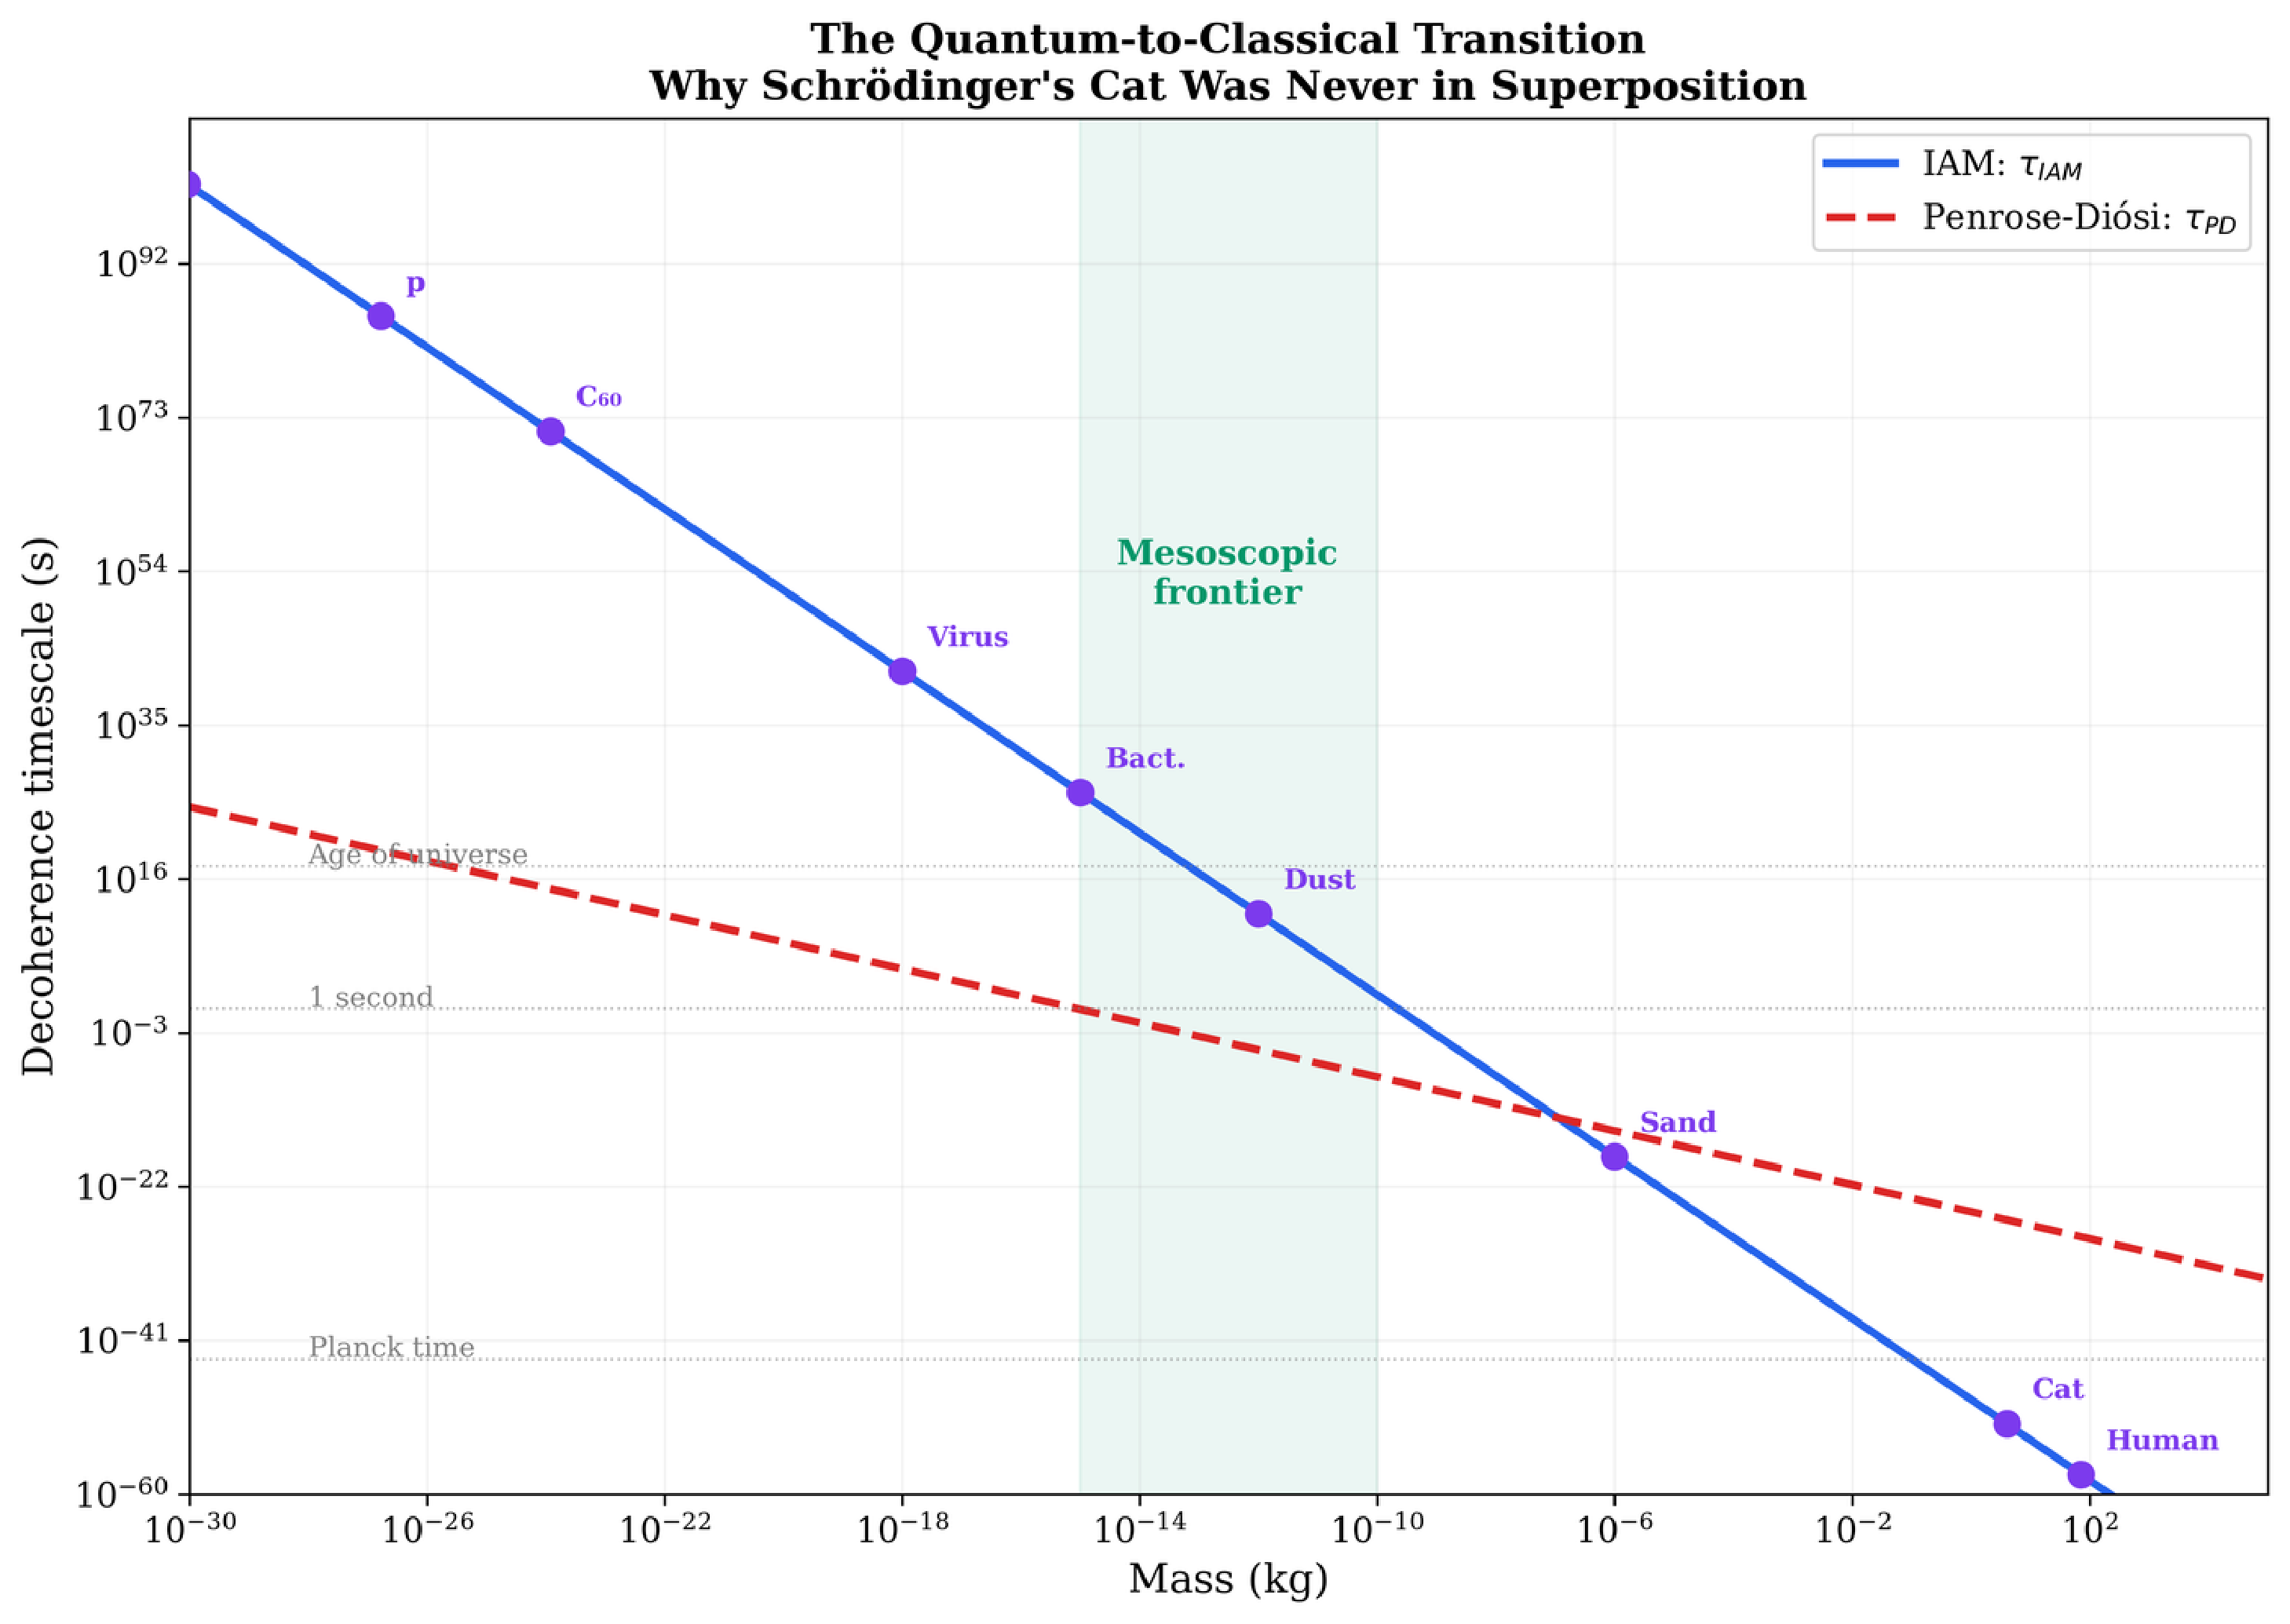
\includegraphics[width=0.88\textwidth]{fig_b2_decoherence_landscape.pdf}
\caption{The quantum-to-classical transition. \IAM{} timescale
$\tauIAM$ (blue) versus Penrose--Di\'{o}si $\tauPD$ (red dashed) for
all objects from electron to human at 300~K. The mesoscopic frontier
(green shaded) marks where predictions are testable. The cat
($\tauIAM \approx 10^{-51}~\text{s}$) decoheres $10^7$ times faster
than the Planck time. It was never in superposition.}
\label{fig:landscape}
\end{figure}

\subsection{Entanglement and Bell Tests}

Entangled particles show correlations that violate Bell inequalities,
seemingly requiring nonlocal connections. \IAM{} provides a local,
causal explanation.

Entangled photons traveling to separated detectors are in the $\Sigma =
1$ sector during transit. They have $\EG = 0$ and $\tauIAM = \infty$.
Their entanglement is preserved not by any nonlocal connection but by
the absence of decoherence during flight. \IAM{} is not a local hidden
variable theory. It preserves the full quantum state during transit and
specifies when the transition from indefinite to definite occurs. The
CHSH $S$-parameter is $|S| = 2\sqrt{2}$, identical to quantum mechanics
and violating the Bell bound of 2.

For matter-based entangled systems, the particles are in the $\mu < 1$
sector during transit and experience gravitational decoherence. The Bell
violation decays as:
\begin{equation}
    S(t) = 2\sqrt{2}\,(1 - D(t)), \quad D(t) = E_q(t/\tauIAM)/e.
    \label{eq:bell}
\end{equation}
When $D$ exceeds 0.293, the Bell violation disappears. Current
experimental records are consistent: photon entanglement at 1,200~km
(Micius satellite, 2017)~\citep{Yin2017} versus matter entanglement
limited to approximately 1.3~m (trapped ions, 2019) --- a ratio of
one million.

\begin{figure}[H]
\centering
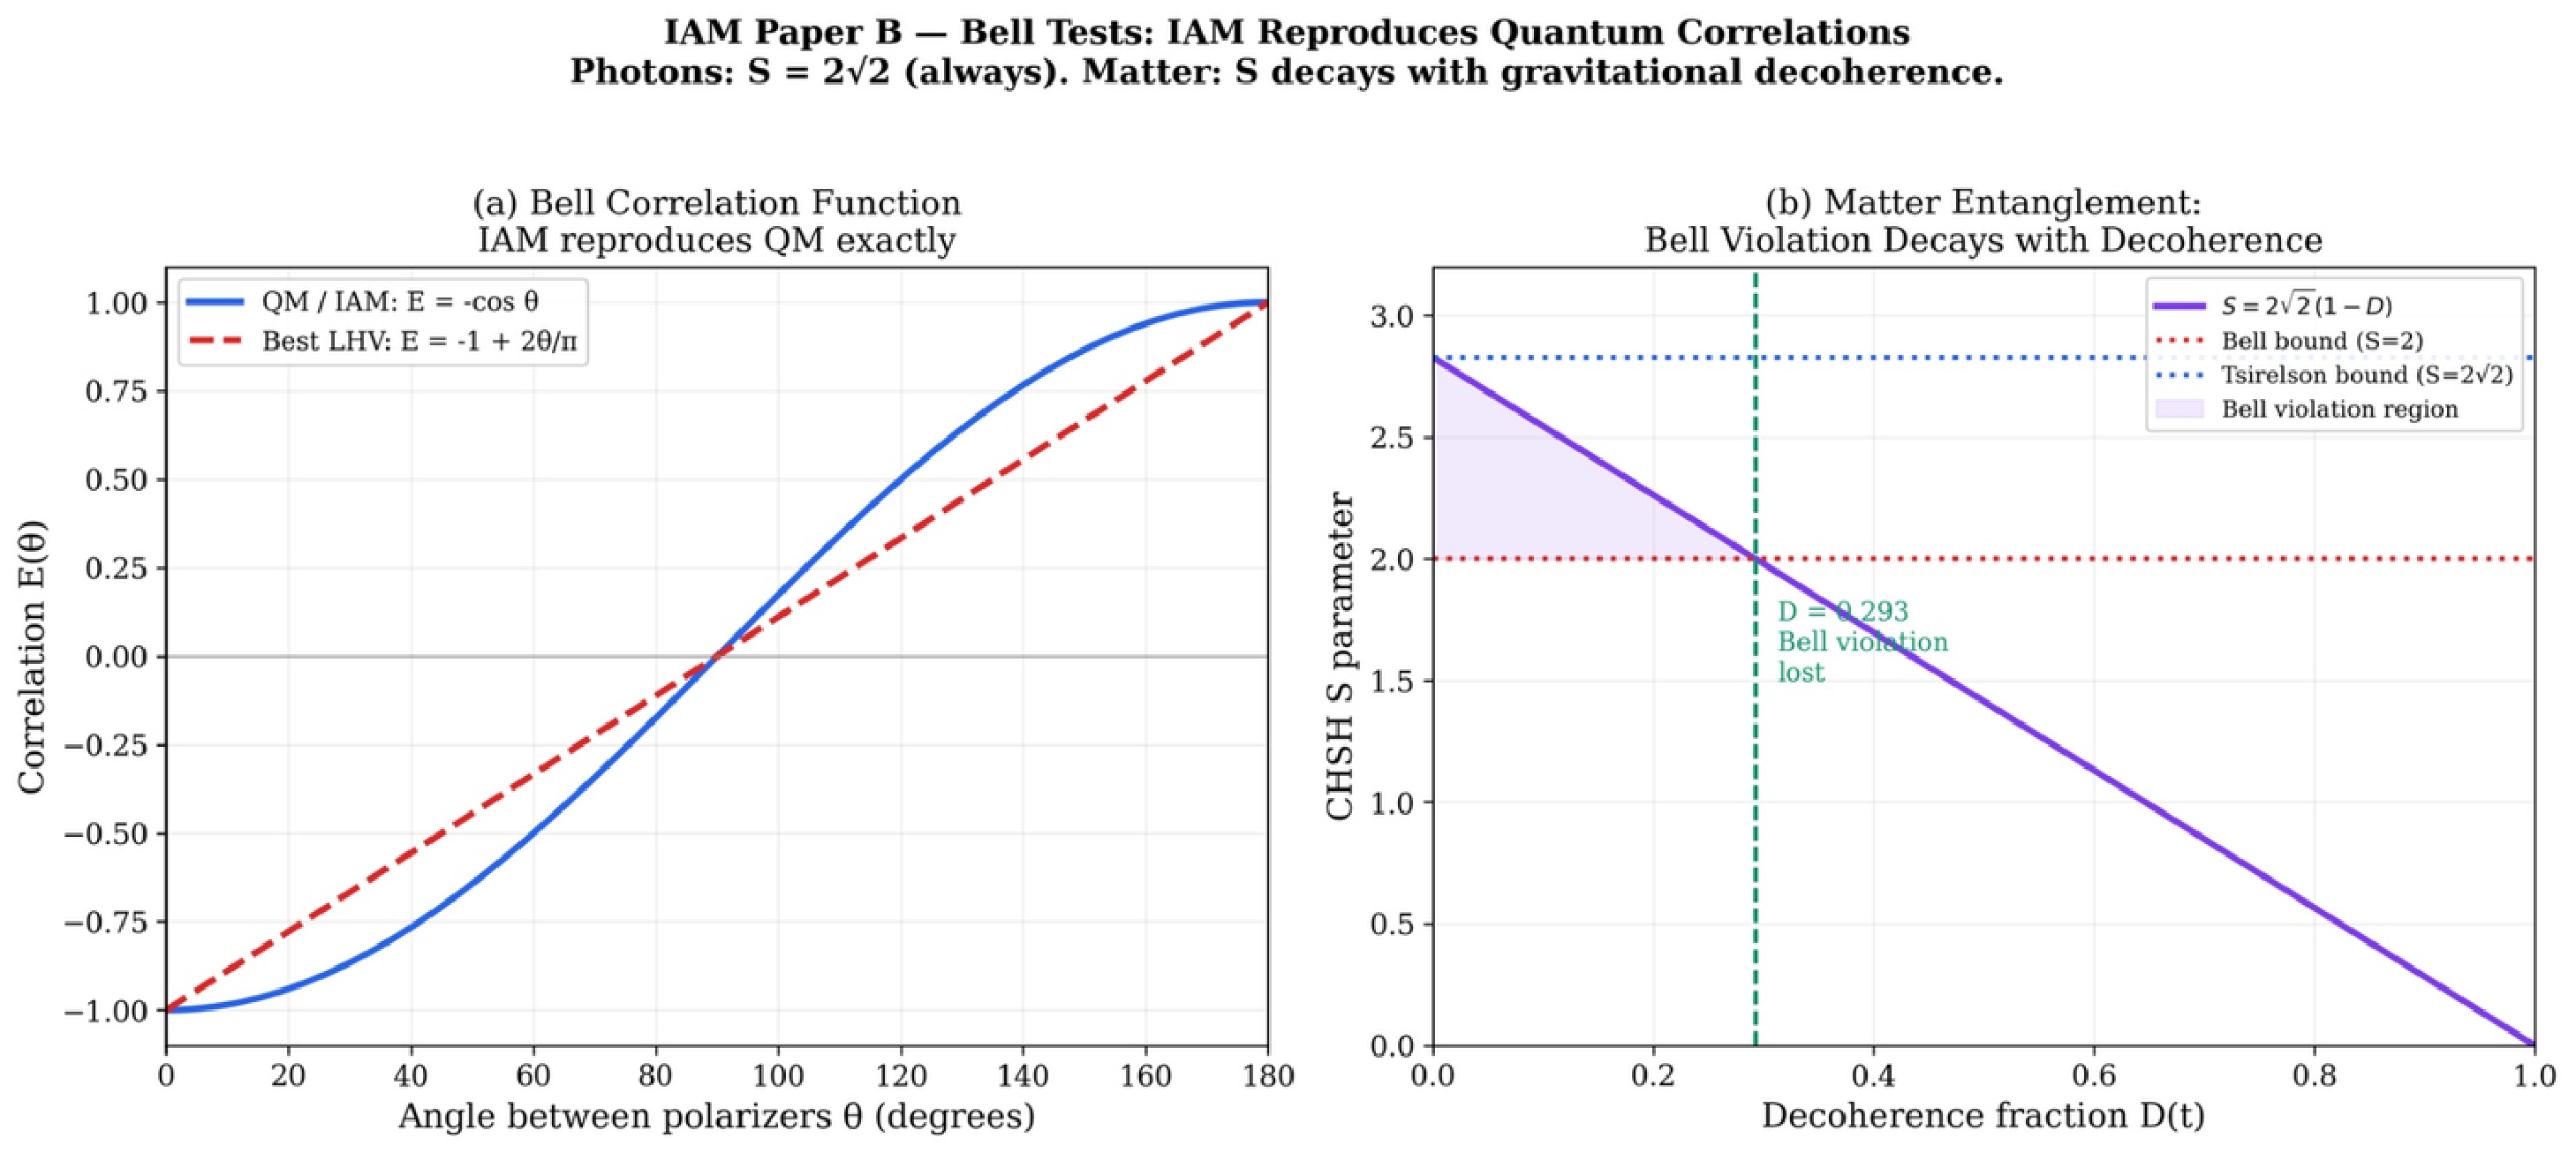
\includegraphics[width=0.88\textwidth]{fig_b5_bell.pdf}
\caption{\textbf{(a)} Bell correlation function: \IAM{} reproduces the
quantum prediction $E(\theta) = -\cos\theta$ exactly. Photons always
maintain $|S| = 2\sqrt{2}$.
\textbf{(b)} Matter entanglement: the CHSH $S$-parameter decays as
$S = 2\sqrt{2}(1-D)$. Bell violation is lost when decoherence fraction
$D > 0.293$ (green dashed line).}
\label{fig:bell}
\end{figure}

\begin{figure}[H]
\centering
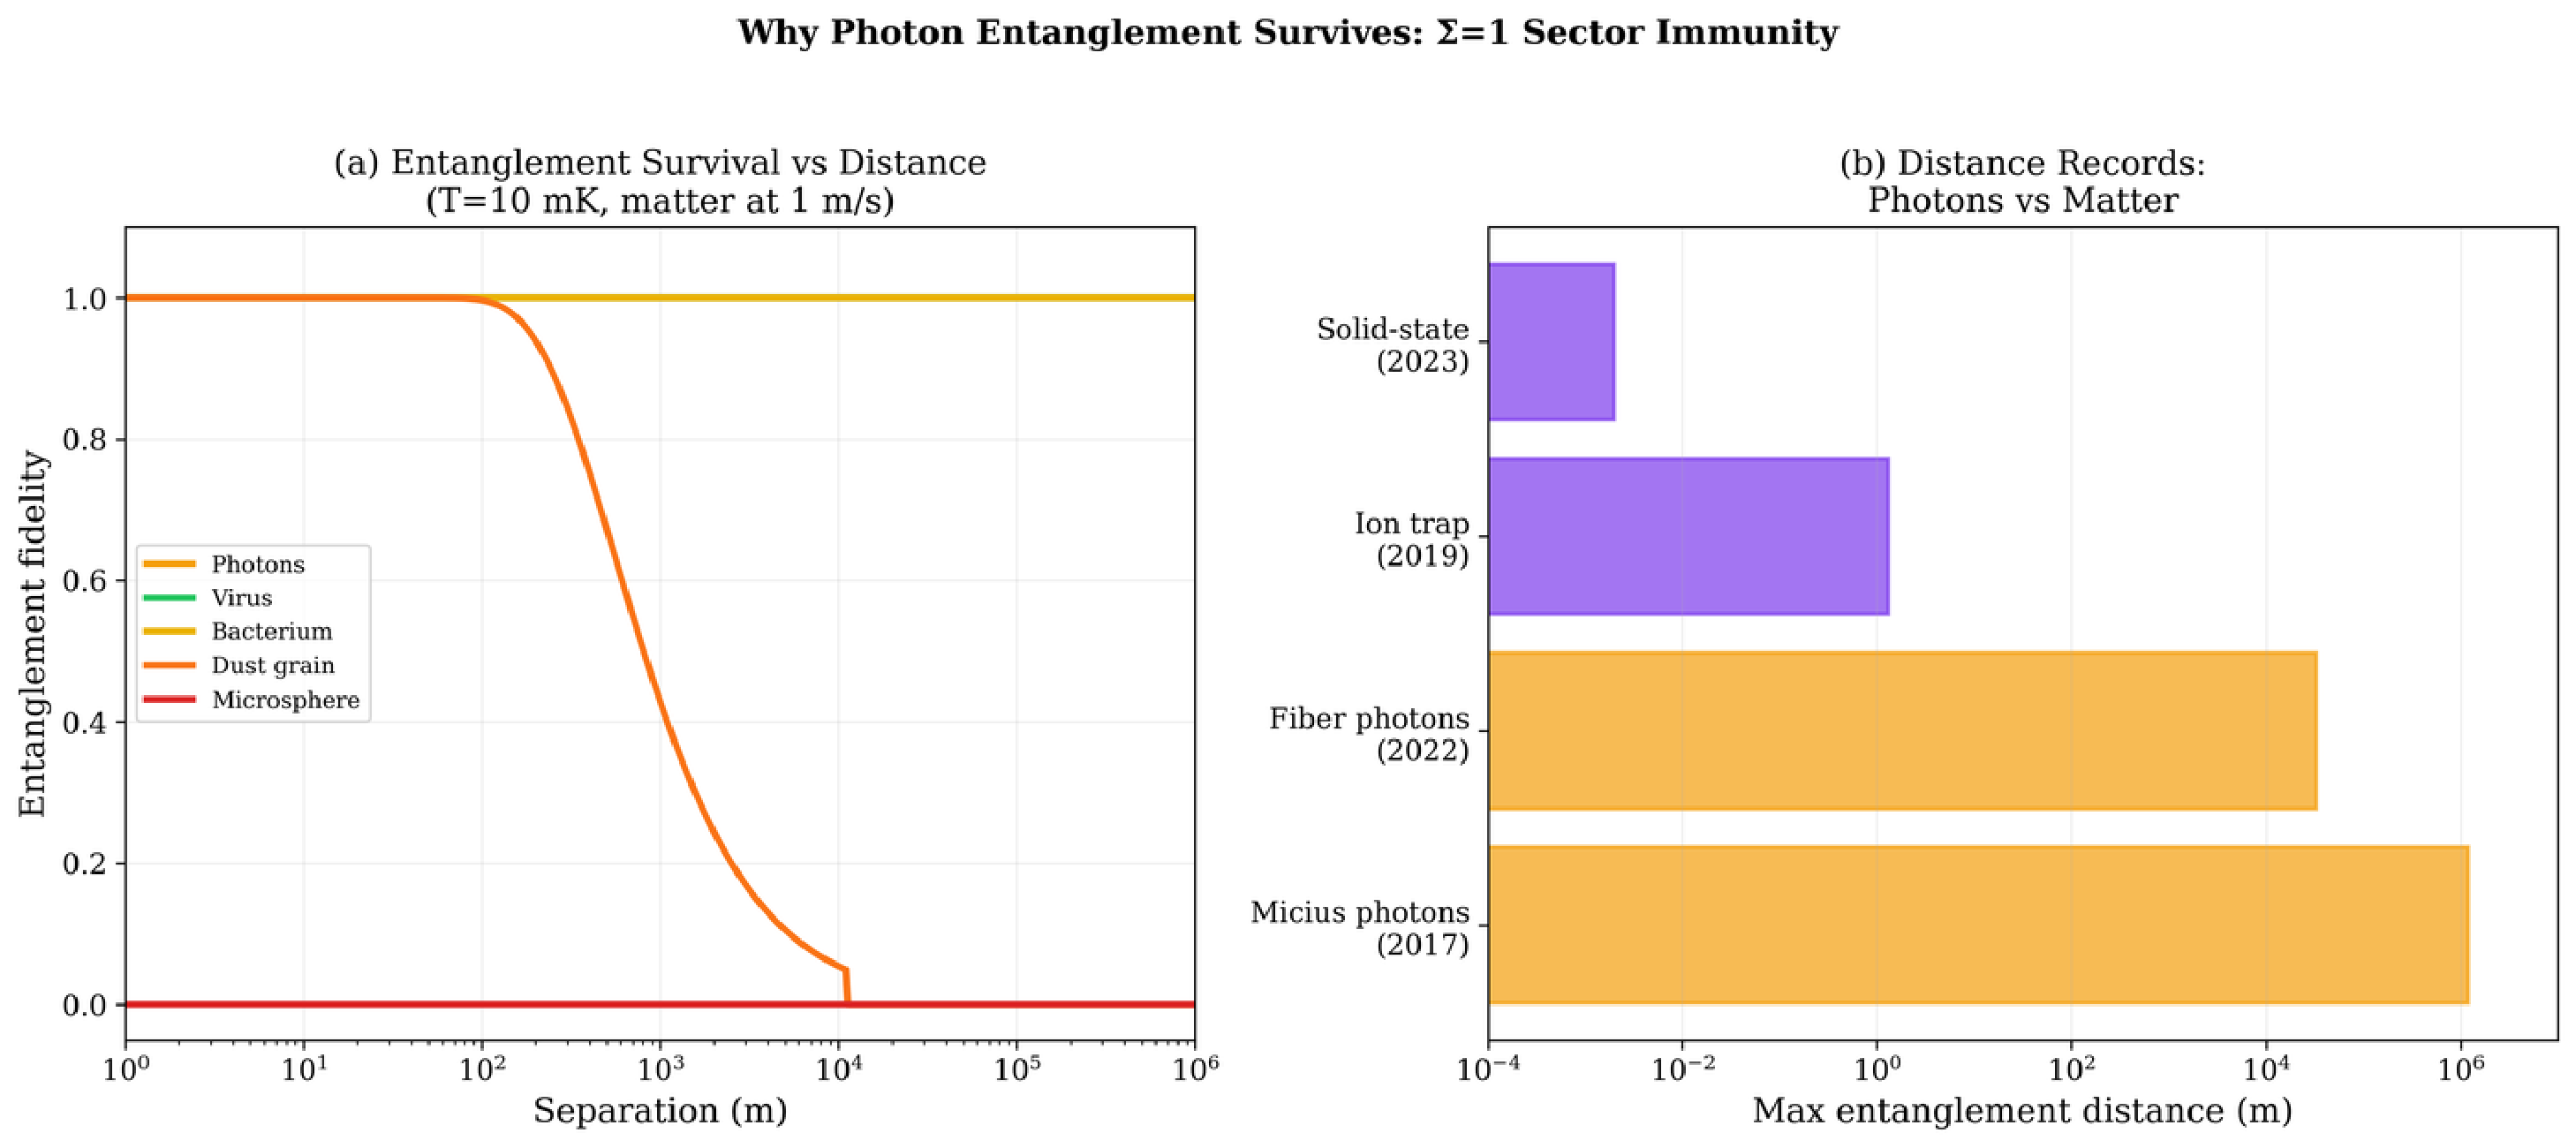
\includegraphics[width=0.88\textwidth]{fig_b4_entanglement.pdf}
\caption{\textbf{(a)} Entanglement fidelity vs.\ separation for
different masses at 10~mK. Photons (orange): fidelity = 1 at any
distance. Matter systems decay at mass-dependent distances.
\textbf{(b)} Experimental distance records: photon entanglement
(Micius, fiber) exceeds matter entanglement (ion trap, solid-state) by
six orders of magnitude, consistent with \IAM{} prediction.}
\label{fig:entanglement}
\end{figure}

\subsection{Wigner's Friend}

In the Wigner's friend scenario, a friend measures a quantum system
inside a sealed lab. Standard quantum mechanics allows Wigner, outside
the lab, to describe the lab (including the friend) as being in a
superposition. Extended scenarios~\citep{Frauchiger2018} show this leads
to logical contradictions.

\IAM{} resolves this by making collapse objective. When the friend's
detector registers a result, it produces irreversible Landauer entropy.
A typical Stern--Gerlach measurement with fluorescent screen produces
approximately 1,000 photons at 2~eV each, representing over $10^5$ bits
of Landauer entropy. The probability of spontaneous reversal is
$2^{-111604} \approx 10^{-33596}$. This is not practically difficult.
It is thermodynamically impossible.

Wigner cannot describe the lab as being in superposition because the
measurement produced irreversible entropy. The collapse was objective
the moment $Q$ exceeded $\QL$. Wigner's knowledge is irrelevant. There
is no paradox because collapse is a physical event (entropy production),
not a mental event (knowledge update).

\begin{figure}[H]
\centering
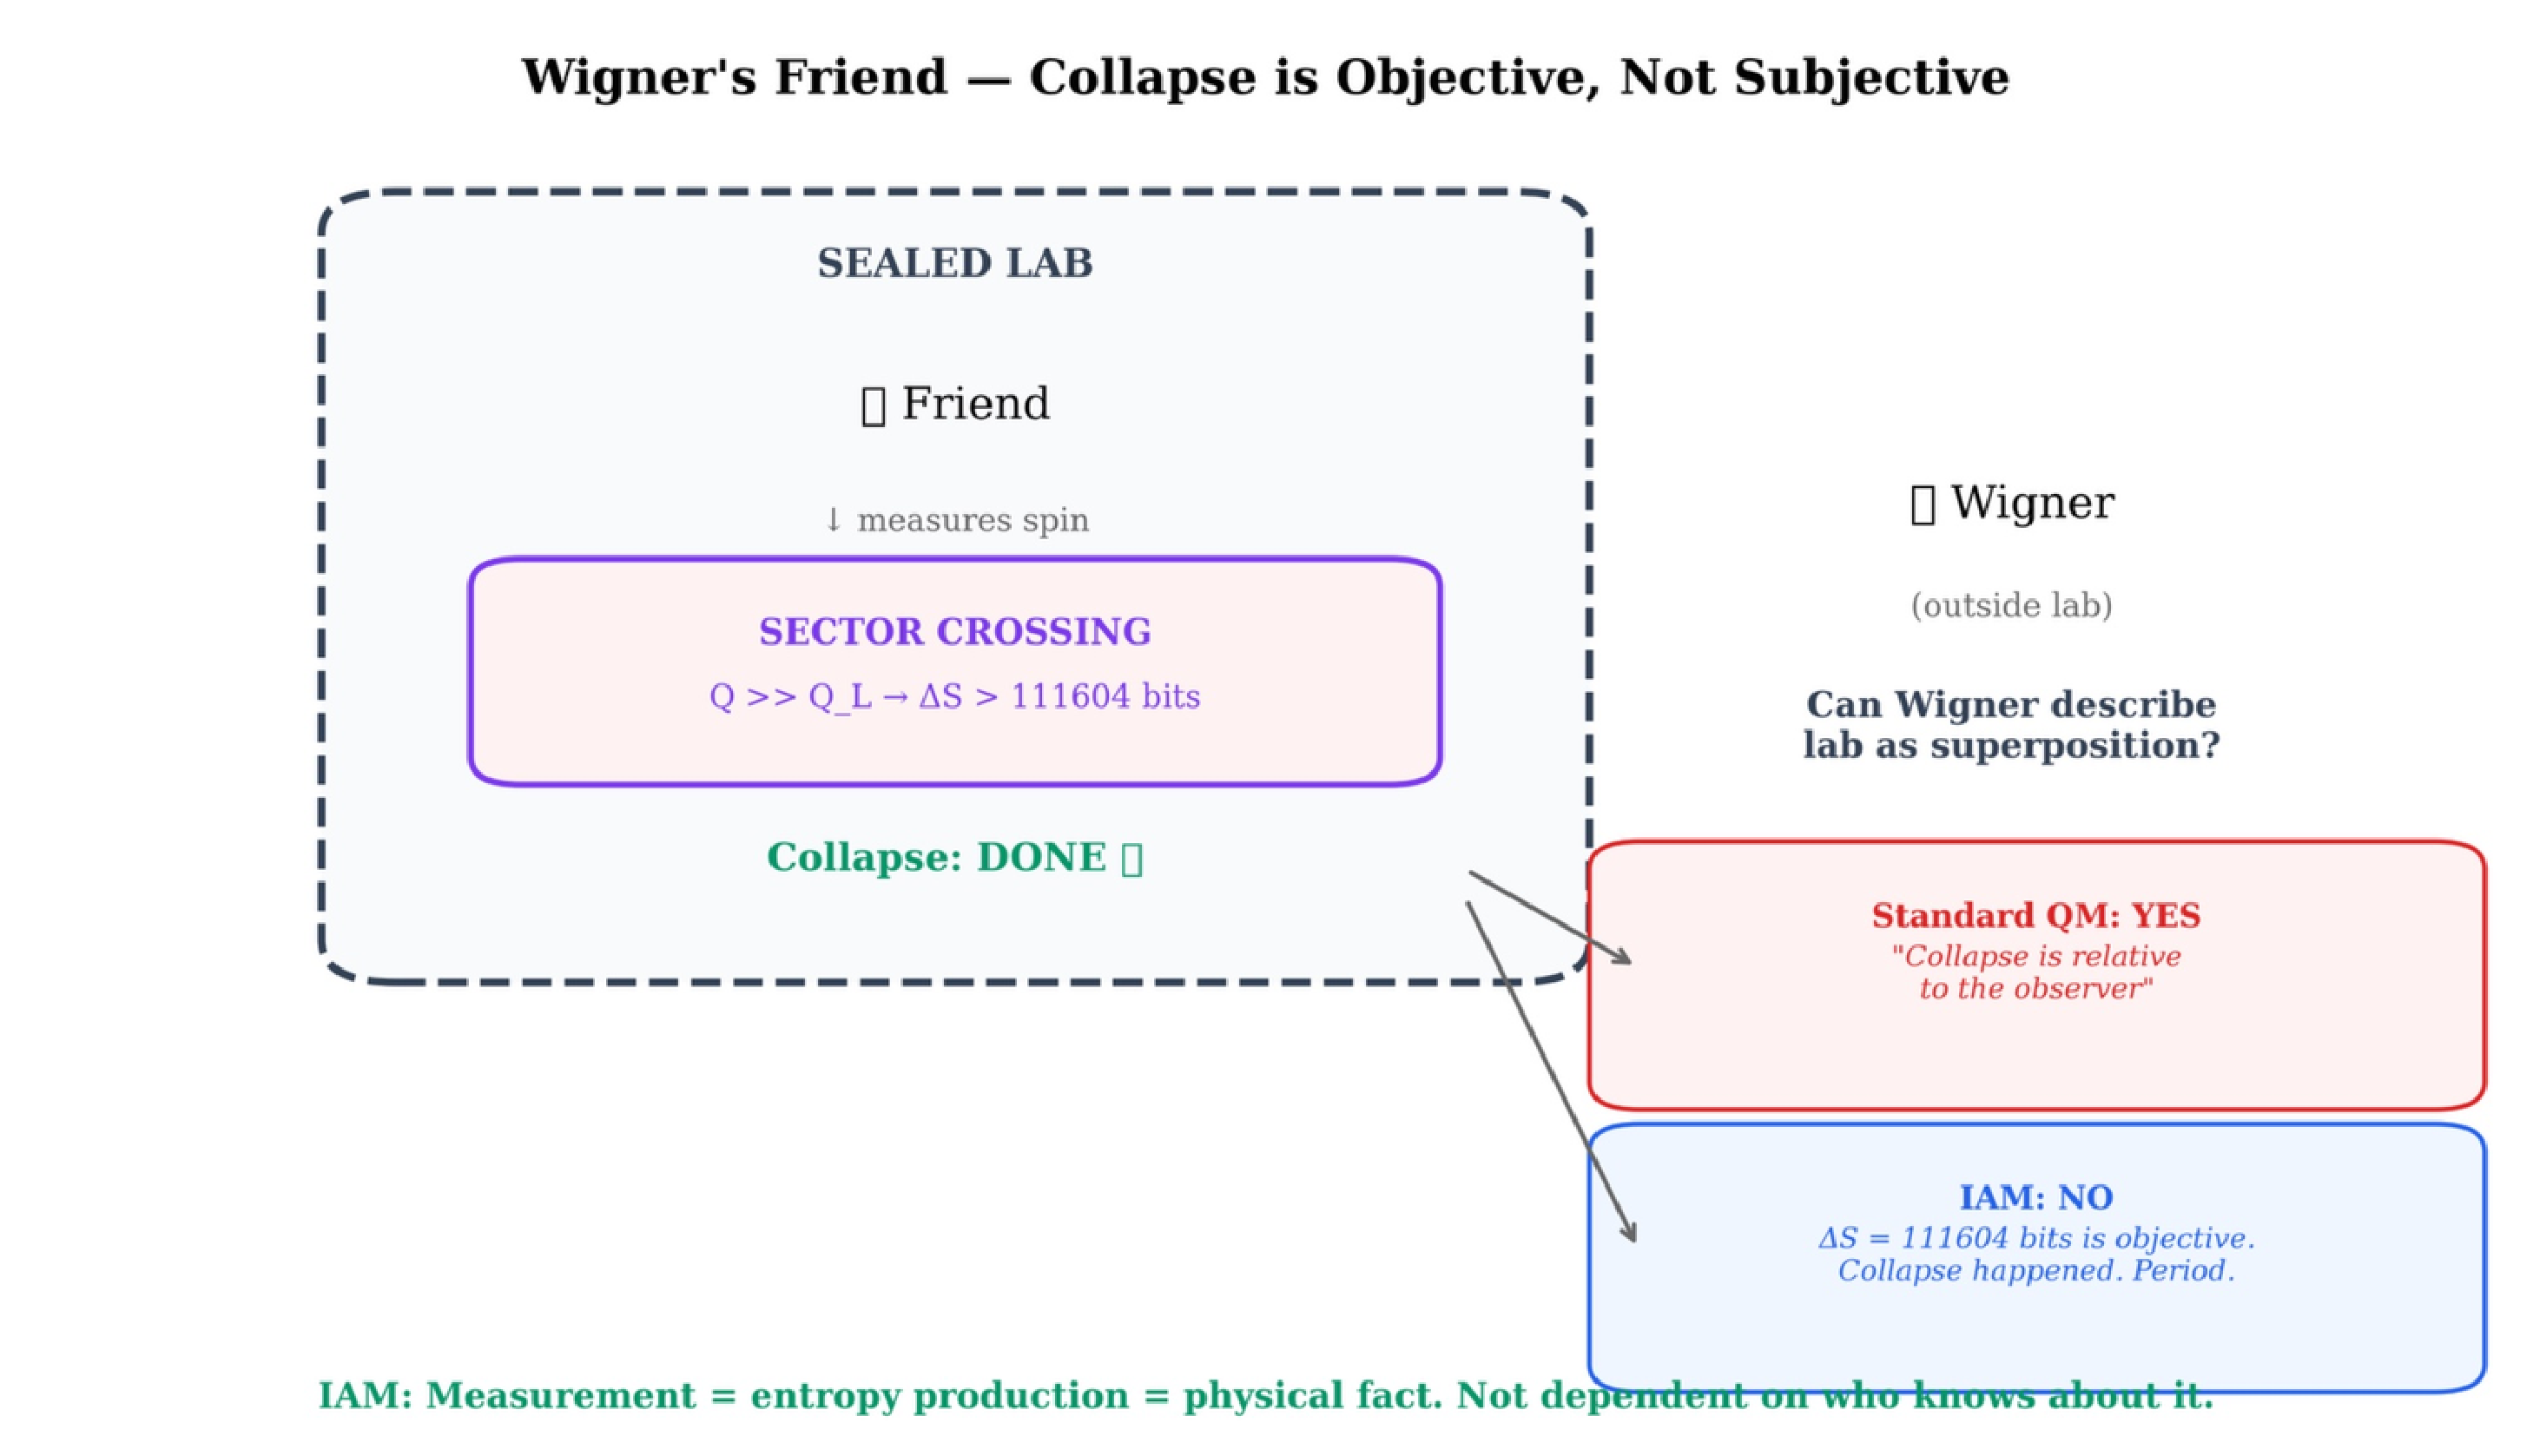
\includegraphics[width=0.80\textwidth]{fig_b6_wigner.pdf}
\caption{Wigner's Friend. When the friend measures spin, the
interaction produces $Q \gg \QL$: sector crossing is objective
($\Delta S > 10^5$ bits). Wigner outside the lab cannot describe the
system as a superposition because the Landauer entropy is a physical
fact. Standard QM: collapse is observer-relative. \IAM{}: collapse is
thermodynamic.}
\label{fig:wigner}
\end{figure}

\subsection{The Quantum Zeno Effect}

The quantum Zeno effect --- frequent measurements freezing a system's
evolution --- has been experimentally confirmed in multiple systems.
Standard quantum mechanics explains it through repeated state projection.

\IAM{} predicts that the Zeno effect requires irreversible measurements.
Each measurement with $Q > \QL$ causes a genuine sector crossing,
resetting the $E_q$ decoherence ramp and interrupting coherent
evolution. Measurements with $Q < \QL$ produce no sector crossing and
should not cause Zeno freezing. This is directly testable with
superconducting qubits, where both dispersive readout (reversible,
$Q \ll \QL$) and destructive readout (irreversible, $Q \gg \QL$) are
available. Standard quantum mechanics predicts both produce the Zeno
effect. \IAM{} predicts only irreversible readout produces Zeno
freezing.

\begin{figure}[H]
\centering
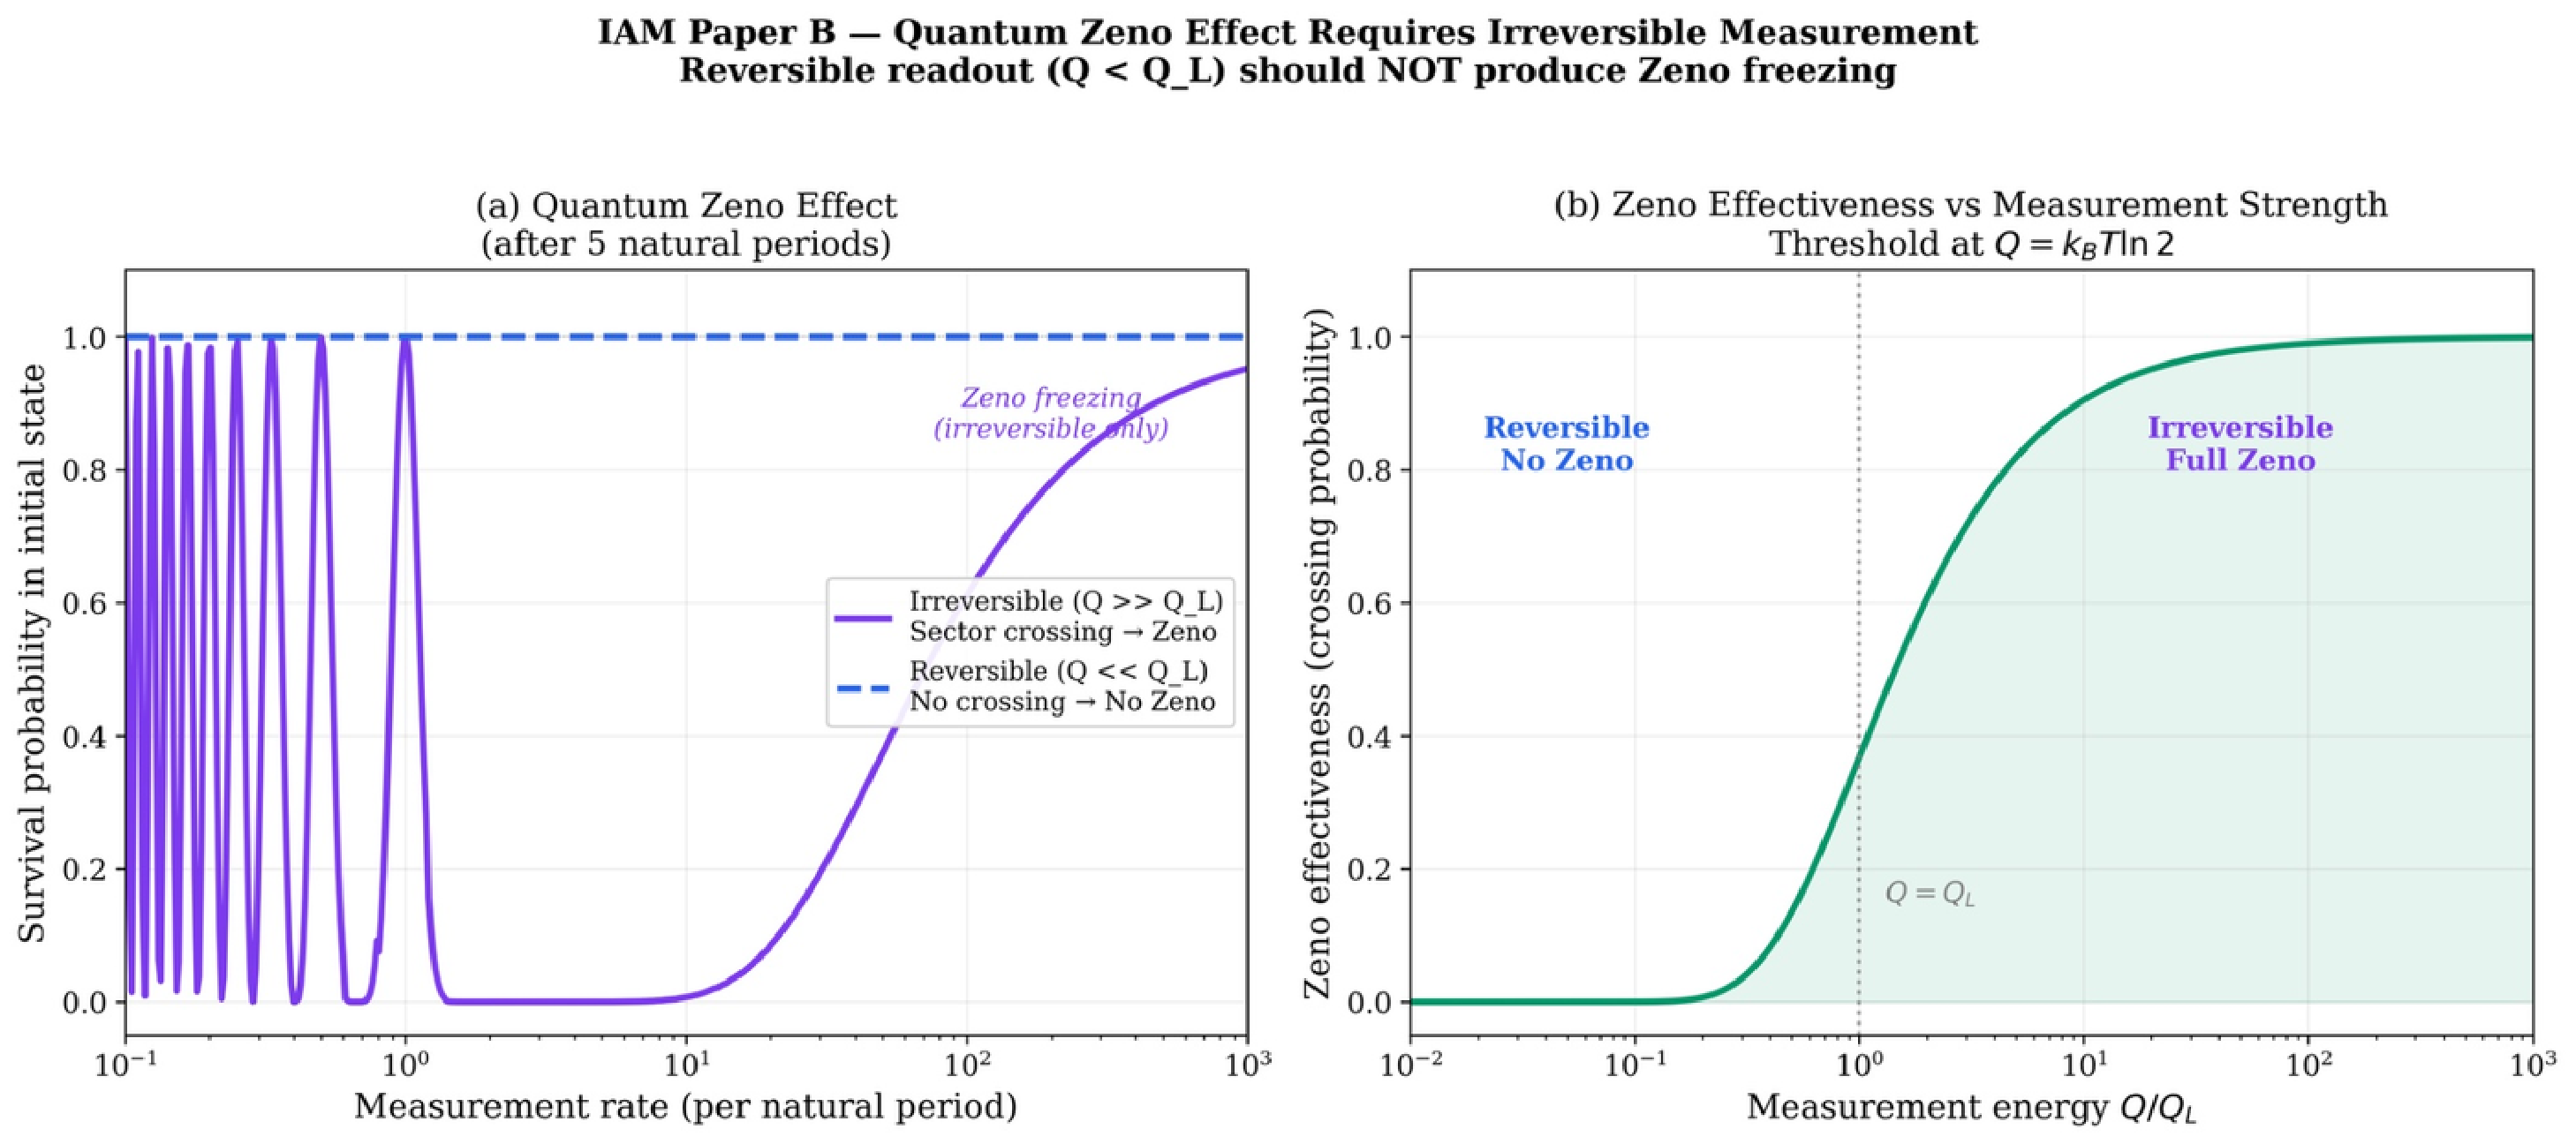
\includegraphics[width=0.88\textwidth]{fig_b7_zeno.pdf}
\caption{\textbf{(a)} Quantum Zeno survival probability after 5
natural periods. Irreversible measurements ($Q \gg \QL$, solid
purple): Zeno freezing at high measurement rate. Reversible
measurements ($Q \ll \QL$, blue dashed): no Zeno effect.
\textbf{(b)} Zeno effectiveness vs.\ $Q/\QL$. The transition
occurs near the Landauer threshold.}
\label{fig:zeno}
\end{figure}

\section{Experimental Predictions}

Three experiments discriminate between \IAM{} and standard quantum
mechanics using existing laboratory infrastructure. All three are
feasible with current technology and require no new hardware.

\subsection{The Two-Detector Quantum Eraser}

Build two versions of the same quantum eraser experiment with identical
photon sources, slits, and detection screens. Version~A uses a
reversible which-path detector (polarization rotation, $Q \ll \QL$).
Version~B uses an irreversible which-path detector (fluorescence or
photodiode, $Q \gg \QL$). Both versions attempt erasure through
conjugate-basis measurement of the ancilla. Standard quantum mechanics
predicts both show restored interference ($F = 1$). \IAM{} predicts
Version~A shows interference and Version~B does not ($F < 0.02$).

\subsection{The Atomic Timing Test}

Use an atomic which-path detector with controllable spontaneous
emission. Place the atom in a high-Q cavity to suppress emission
(Purcell effect). Vary the delay between which-path marking and erasure
attempt. Standard quantum mechanics predicts interference visibility
independent of delay. \IAM{} predicts a step function: visibility drops
at the spontaneous emission time ($\tau_{\rm emission} \approx
10~\text{ns}$) as the emitted photon carries $Q = 2~\text{eV} \gg \QL$
irreversibly into the environment.

\subsection{The Temperature Test}

Run the same quantum eraser at multiple temperatures. The Landauer
threshold $\QL = \kB T \ln 2$ depends linearly on temperature. Standard
quantum mechanics predicts no temperature dependence. \IAM{} predicts
erasure fidelity increases with temperature because a higher $\QL$
makes it harder for the which-path interaction to be irreversible. For
a 0.1~eV interaction energy: $F = 0.000$ at 10~mK, $F = 0.002$ at
4~K, and $F = 0.164$ at 300~K.

\begin{figure}[H]
\centering
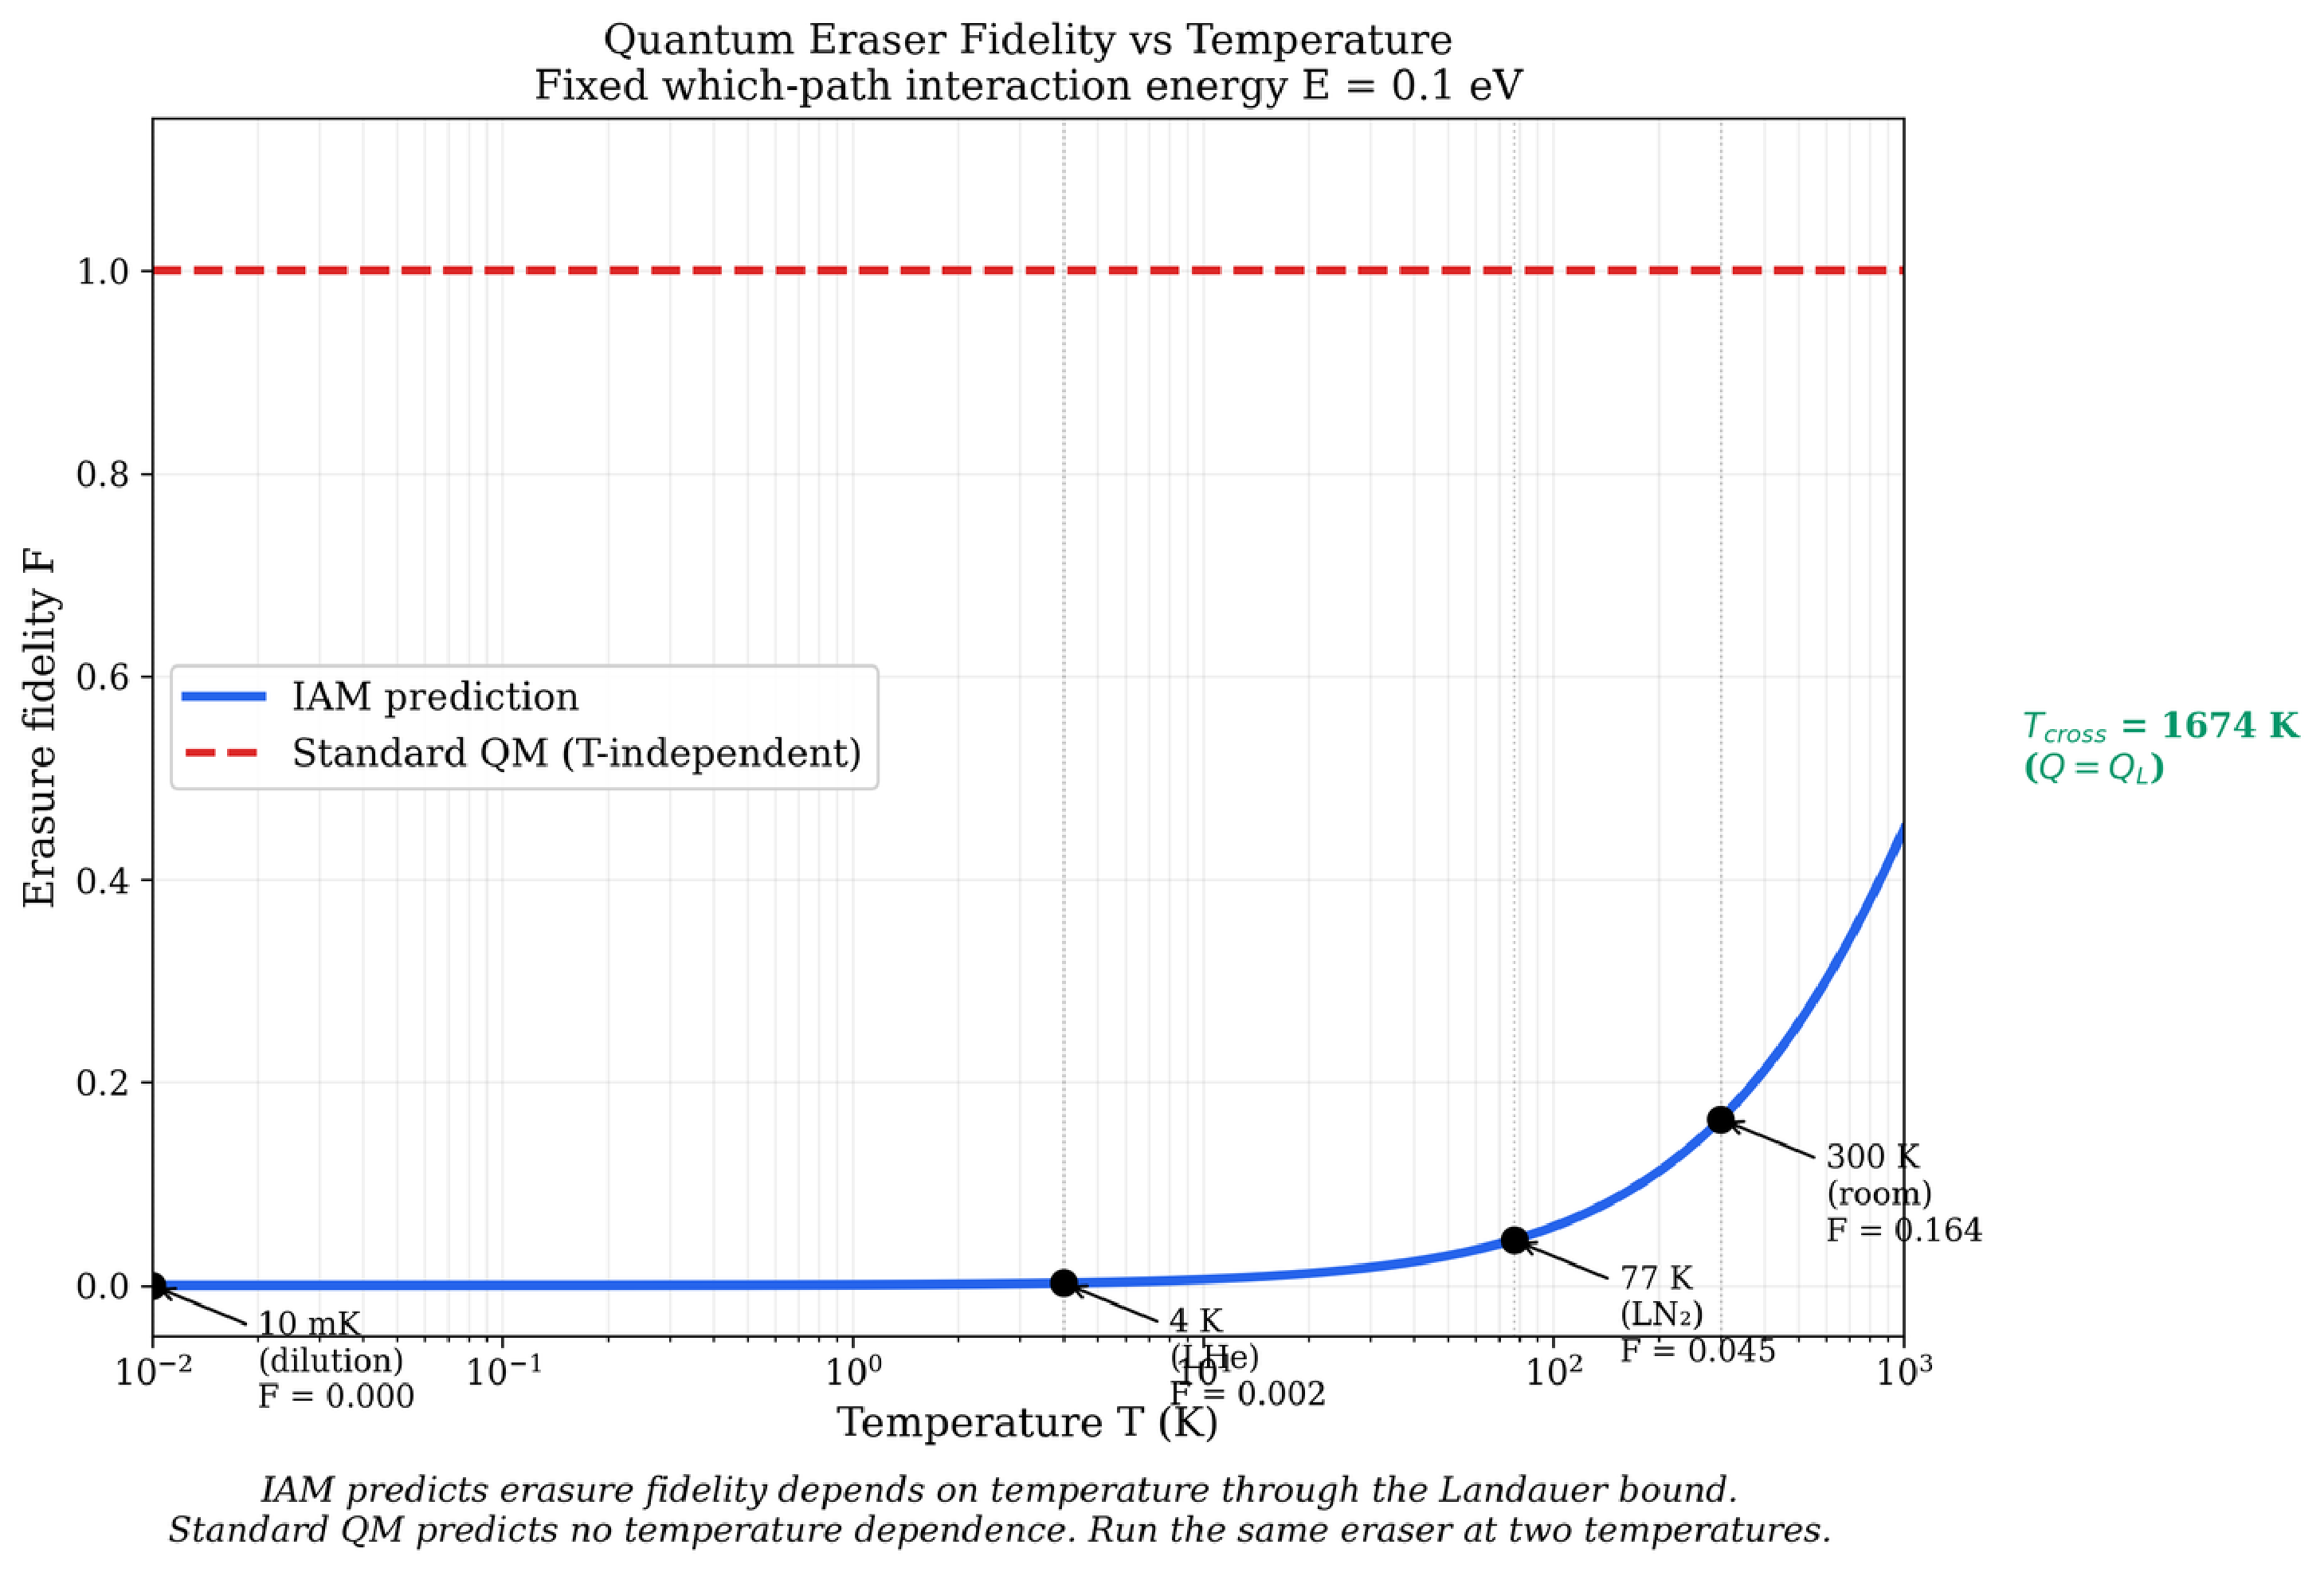
\includegraphics[width=0.80\textwidth]{fig_eraser_temperature.pdf}
\caption{Erasure fidelity vs.\ temperature for a fixed which-path
interaction energy of 0.1~eV. \IAM{} (blue): strong temperature
dependence through the Landauer bound. Standard QM (red dashed): no
temperature dependence. Running the same eraser at 10~mK and 300~K
provides a clean discrimination test.}
\label{fig:eraser_temperature}
\end{figure}

\section{Connection to Cosmological Validation}

The sector crossing mechanism that governs quantum decoherence is the
same physical process that, accumulated over approximately $10^{11}$
galaxies and 13.8~billion years, produces the informational entropy that
modifies cosmic expansion. At cosmological scales, the cumulative
integral of irreversible gravitational information production yields
$E(a) = \exp(1 - 1/a)$, modifying the matter-sector perturbation
equations and producing the signature $\mu < 1$, $\Sigma = 1$. At
quantum scales, the same integral yields $E_q(\eta) = \exp(1 - 1/\eta)$,
governing the decoherence profile of individual mesoscopic systems.

The laboratory experiment measures the rate per decoherence event.
Cosmology measures the cumulative effect. Consistency between the two ---
cosmological data preferring $\mu < 1$ with the correct redshift
dependence and laboratory data showing the $E_q$ ramp profile at the
predicted $\tauIAM$ --- would close the loop from quantum mechanics to
the accelerating universe through the same equation, the same
thermodynamics, and the same physics at every scale.

\section{Discussion}

\subsection{Relationship to Existing Interpretations}

\IAM's resolution of the measurement problem shares elements with
several existing approaches while differing from each in important ways.
Like decoherence theory~\citep{Zurek2003}, \IAM{} identifies
environmental interaction as the mechanism for apparent collapse. Unlike
decoherence theory, \IAM{} specifies the precise threshold
($\QL = \kB T \ln 2$) and predicts qualitatively different outcomes for
reversible versus irreversible interactions. Like objective collapse
models~\citep{Penrose1996,Diosi1987}, \IAM{} predicts that collapse is
a physical process independent of observers. Unlike those models, \IAM{}
does not introduce new stochastic fields or modify the
Schr\"{o}dinger equation.

\subsection{What IAM Does Not Change}

\IAM{} does not modify the predictions of quantum mechanics for any
experiment that has been performed to date. All existing quantum eraser
experiments use reversible which-path detectors (polarization
entanglement via BBO crystals) and both models predict successful
erasure. All existing Bell tests use photonic entanglement and both
models predict $|S| = 2\sqrt{2}$. The Zeno effect has been demonstrated
with projective measurements that are thermodynamically irreversible,
and both models predict Zeno freezing. The predictions diverge only for
experiments not yet performed.

\subsection{Falsification}

If irreversible which-path detection ($Q \gg \QL$) still allows
successful quantum erasure, \IAM's Landauer criterion is falsified at
the quantum scale. If the Zeno effect is observed with
thermodynamically reversible measurements ($Q \ll \QL$), the sector
crossing mechanism is falsified. If matter entanglement shows no
mass-dependent or distance-dependent degradation beyond environmental
predictions, the gravitational decoherence mechanism is excluded.

\section{Conclusion}

The measurement problem is dissolved by recognizing that ``measurement''
is not a primitive concept but a thermodynamic process: irreversible
sector crossing governed by Landauer's principle. The dual-sector
framework of \IAM, independently validated at cosmological scales
through 17 converged Planck~2018 MCMC chains ($\Delta\chi^2 = +0.54$),
provides the quantitative criterion ($Q \geq \kB T \ln 2$) that standard
quantum mechanics leaves undefined. This single criterion resolves the
double slit, delayed choice, quantum eraser, Schr\"{o}dinger's cat,
entanglement, Wigner's friend, and the Zeno effect through the same
physical mechanism. Three experimental tests using existing laboratory
infrastructure can discriminate between \IAM{} and standard quantum
mechanics. The same thermodynamic process that governs decoherence at
quantum scales drives cosmic expansion at cosmological scales. The
measurement problem and the accelerating universe are manifestations of
the same physics.

\section*{Acknowledgments}

The author thanks the developers of CAMB, MGCAMB, and Cobaya for making
cosmological validation accessible to independent researchers. All MCMC
chains, configuration files, modified Fortran source code, and analysis
scripts are publicly archived at
\url{https://github.com/hmahaffeyges/IAM-Validation}.
DOI: \href{https://doi.org/10.17605/OSF.IO/KCZD9}{10.17605/OSF.IO/KCZD9}.

\bibliographystyle{plainnat}
\begin{thebibliography}{99}

\bibitem{Mahaffey2026a}
H.~W. Mahaffey,
``Constraints on Late-Time $f\sigma_8$ Suppression from $\mu < 1$,
$\Sigma = 1$: Planck~2018 and Large-Scale Structure,''
submitted (2026). Manuscript ID: universe-4189350.

\bibitem{Mahaffey2026repo}
H.~W. Mahaffey,
IAM Validation Repository (2026).
\url{https://github.com/hmahaffeyges/IAM-Validation}.
DOI: \href{https://doi.org/10.17605/OSF.IO/KCZD9}{10.17605/OSF.IO/KCZD9}.

\bibitem{Mahaffey2026decoherence}
H.~W. Mahaffey,
``Gravitational Decoherence from Dual-Sector Thermodynamics,''
in preparation (2026) [Paper~8].

\bibitem{Landauer1961}
R.~Landauer,
``Irreversibility and Heat Generation in the Computing Process,''
\textit{IBM J.\ Res.\ Dev.}\ \textbf{5}, 183 (1961).

\bibitem{Penrose1996}
R.~Penrose,
``On Gravity's Role in Quantum State Reduction,''
\textit{Gen.\ Relativ.\ Gravit.}\ \textbf{28}, 581 (1996).

\bibitem{Diosi1987}
L.~Di\'{o}si,
``A Universal Master Equation for the Gravitational Violation of Quantum
Mechanics,''
\textit{Phys.\ Lett.\ A}\ \textbf{120}, 377 (1987).

\bibitem{Zurek2003}
W.~H. Zurek,
``Decoherence, Einselection, and the Quantum Origins of the Classical,''
\textit{Rev.\ Mod.\ Phys.}\ \textbf{75}, 715 (2003).

\bibitem{Yin2017}
J.~Yin et al.,
``Satellite-Based Entanglement Distribution over 1200 Kilometers,''
\textit{Science}\ \textbf{356}, 1140 (2017).

\bibitem{Frauchiger2018}
D.~Frauchiger and R.~Renner,
``Quantum Theory Cannot Consistently Describe the Use of Itself,''
\textit{Nat.\ Commun.}\ \textbf{9}, 3711 (2018).

\bibitem{Jacobson1995}
T.~Jacobson,
``Thermodynamics of Spacetime: The Einstein Equation of State,''
\textit{Phys.\ Rev.\ Lett.}\ \textbf{75}, 1260 (1995).

\bibitem{Wheeler1978}
J.~A. Wheeler,
``The `Past' and the `Delayed-Choice' Double-Slit Experiment,''
in \textit{Mathematical Foundations of Quantum Theory} (1978).

\bibitem{Planck2018}
Planck Collaboration,
``Planck 2018 Results. VI. Cosmological Parameters,''
\textit{Astron.\ Astrophys.}\ \textbf{641}, A6 (2020).

\end{thebibliography}

\end{document}
